%----------------------------------------
\section{Advanced Learning Algorithms}
%----------------------------------------

Building upon the foundational regression and classification models, this course delves into high-capacity models capable of capturing complex, non-linear patterns. It moves from the theoretical underpinnings of Neural Networks to the practical methodology of building, diagnosing, and optimizing real-world machine learning systems.

\begin{figure}[H]
    \centering
    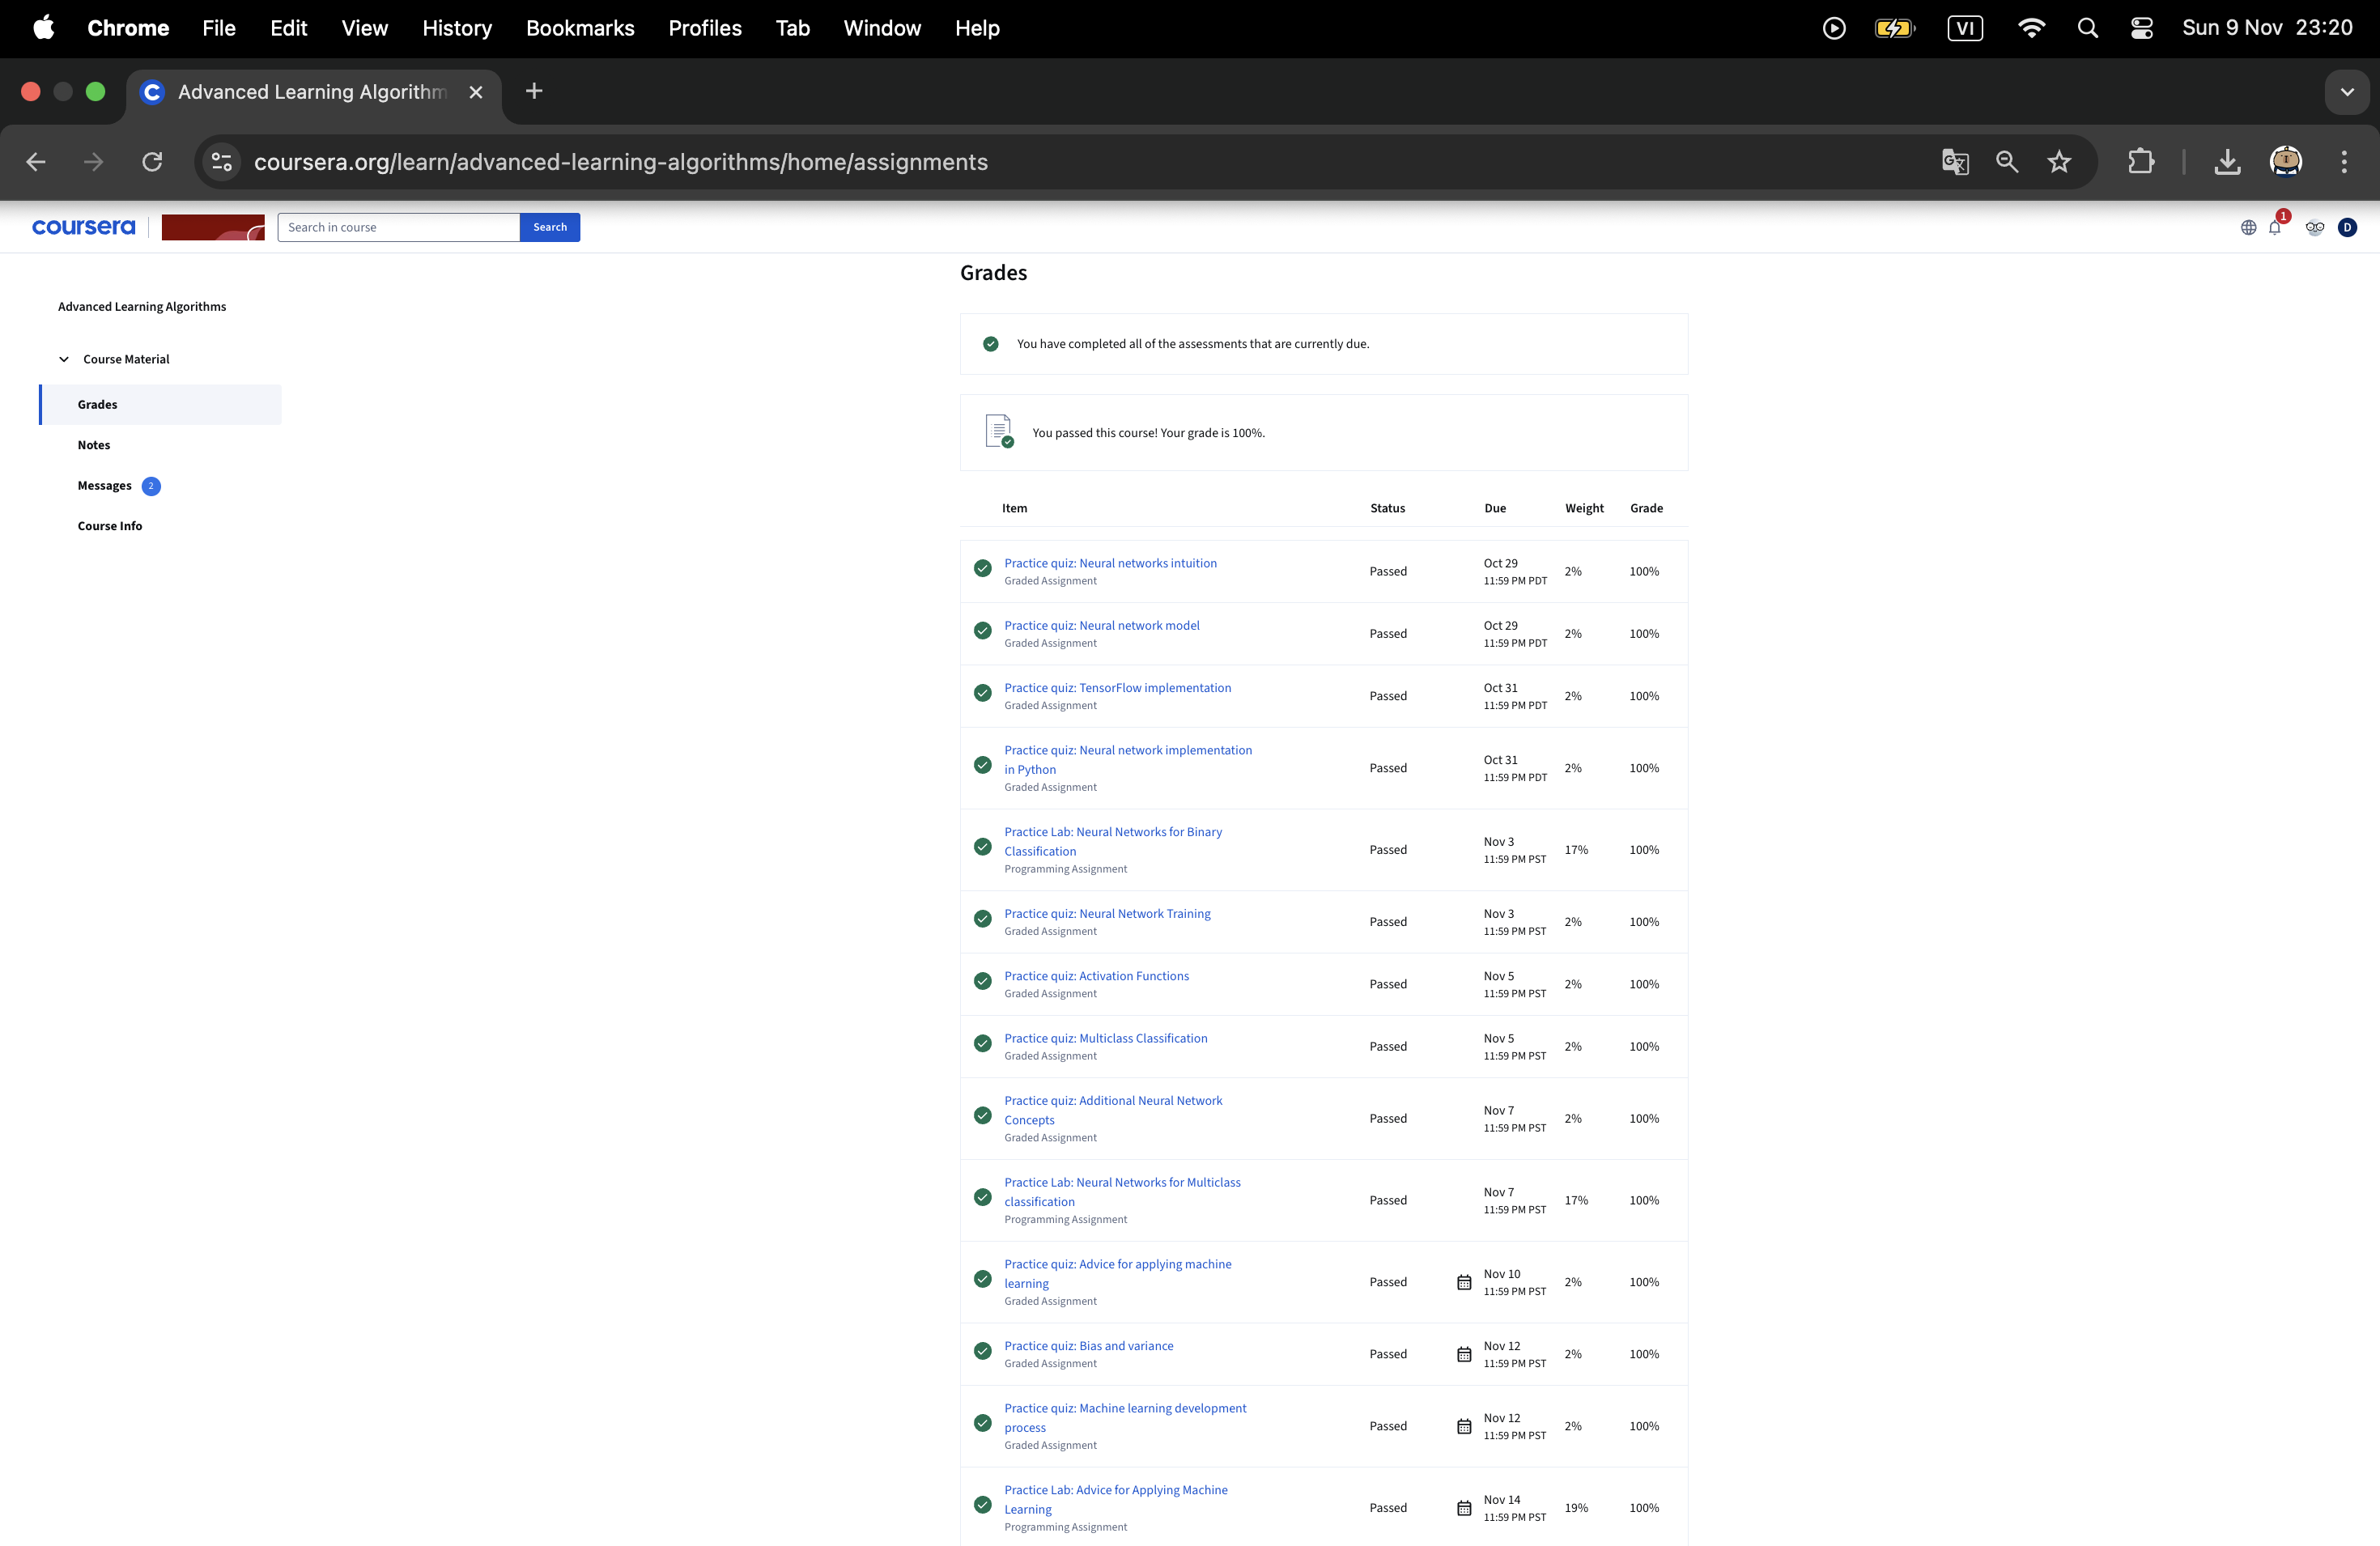
\includegraphics[scale=0.3]{Image/c2.png}
    \caption{Course 2 completed}
\end{figure}

%----------------------------------------
\subsection{Week 1: Neural Networks}
%----------------------------------------

\subsubsection{Key Insights and Learnings}

This module marked the transition from traditional algorithms to Deep Learning, utilizing biological inspiration to solve complex computational problems.

\begin{itemize}
    \item \textbf{Neural Network Architecture:} Understood how stacking layers of logistic regression units creates a "Multi-Layer Perceptron."
    \begin{itemize}
        \item \textbf{Activation Functions:} Analyzed the role of non-linear functions like \textbf{ReLU} (Rectified Linear Unit) for hidden layers to avoid the "vanishing gradient" problem and \textbf{Sigmoid} for binary output.
        \item \textbf{Vectorization:} Leveraged matrix multiplication (via TensorFlow/NumPy) to perform forward propagation efficiently over large datasets.
    \end{itemize}

    \item \textbf{Multiclass Classification (Softmax):} Extended binary classification to multiple categories using the \textbf{Softmax Regression} function, which outputs a probability distribution across $N$ classes (ensuring $\sum P(y=k) = 1$).
    
    \item \textbf{Hierarchical Feature Learning:} Recognized that deep networks learn representations hierarchically—lower layers detect simple edges, while deeper layers assemble them into complex shapes and objects.
\end{itemize}

\subsubsection{Learning Evidence}
\begin{figure}[H]
    \centering
    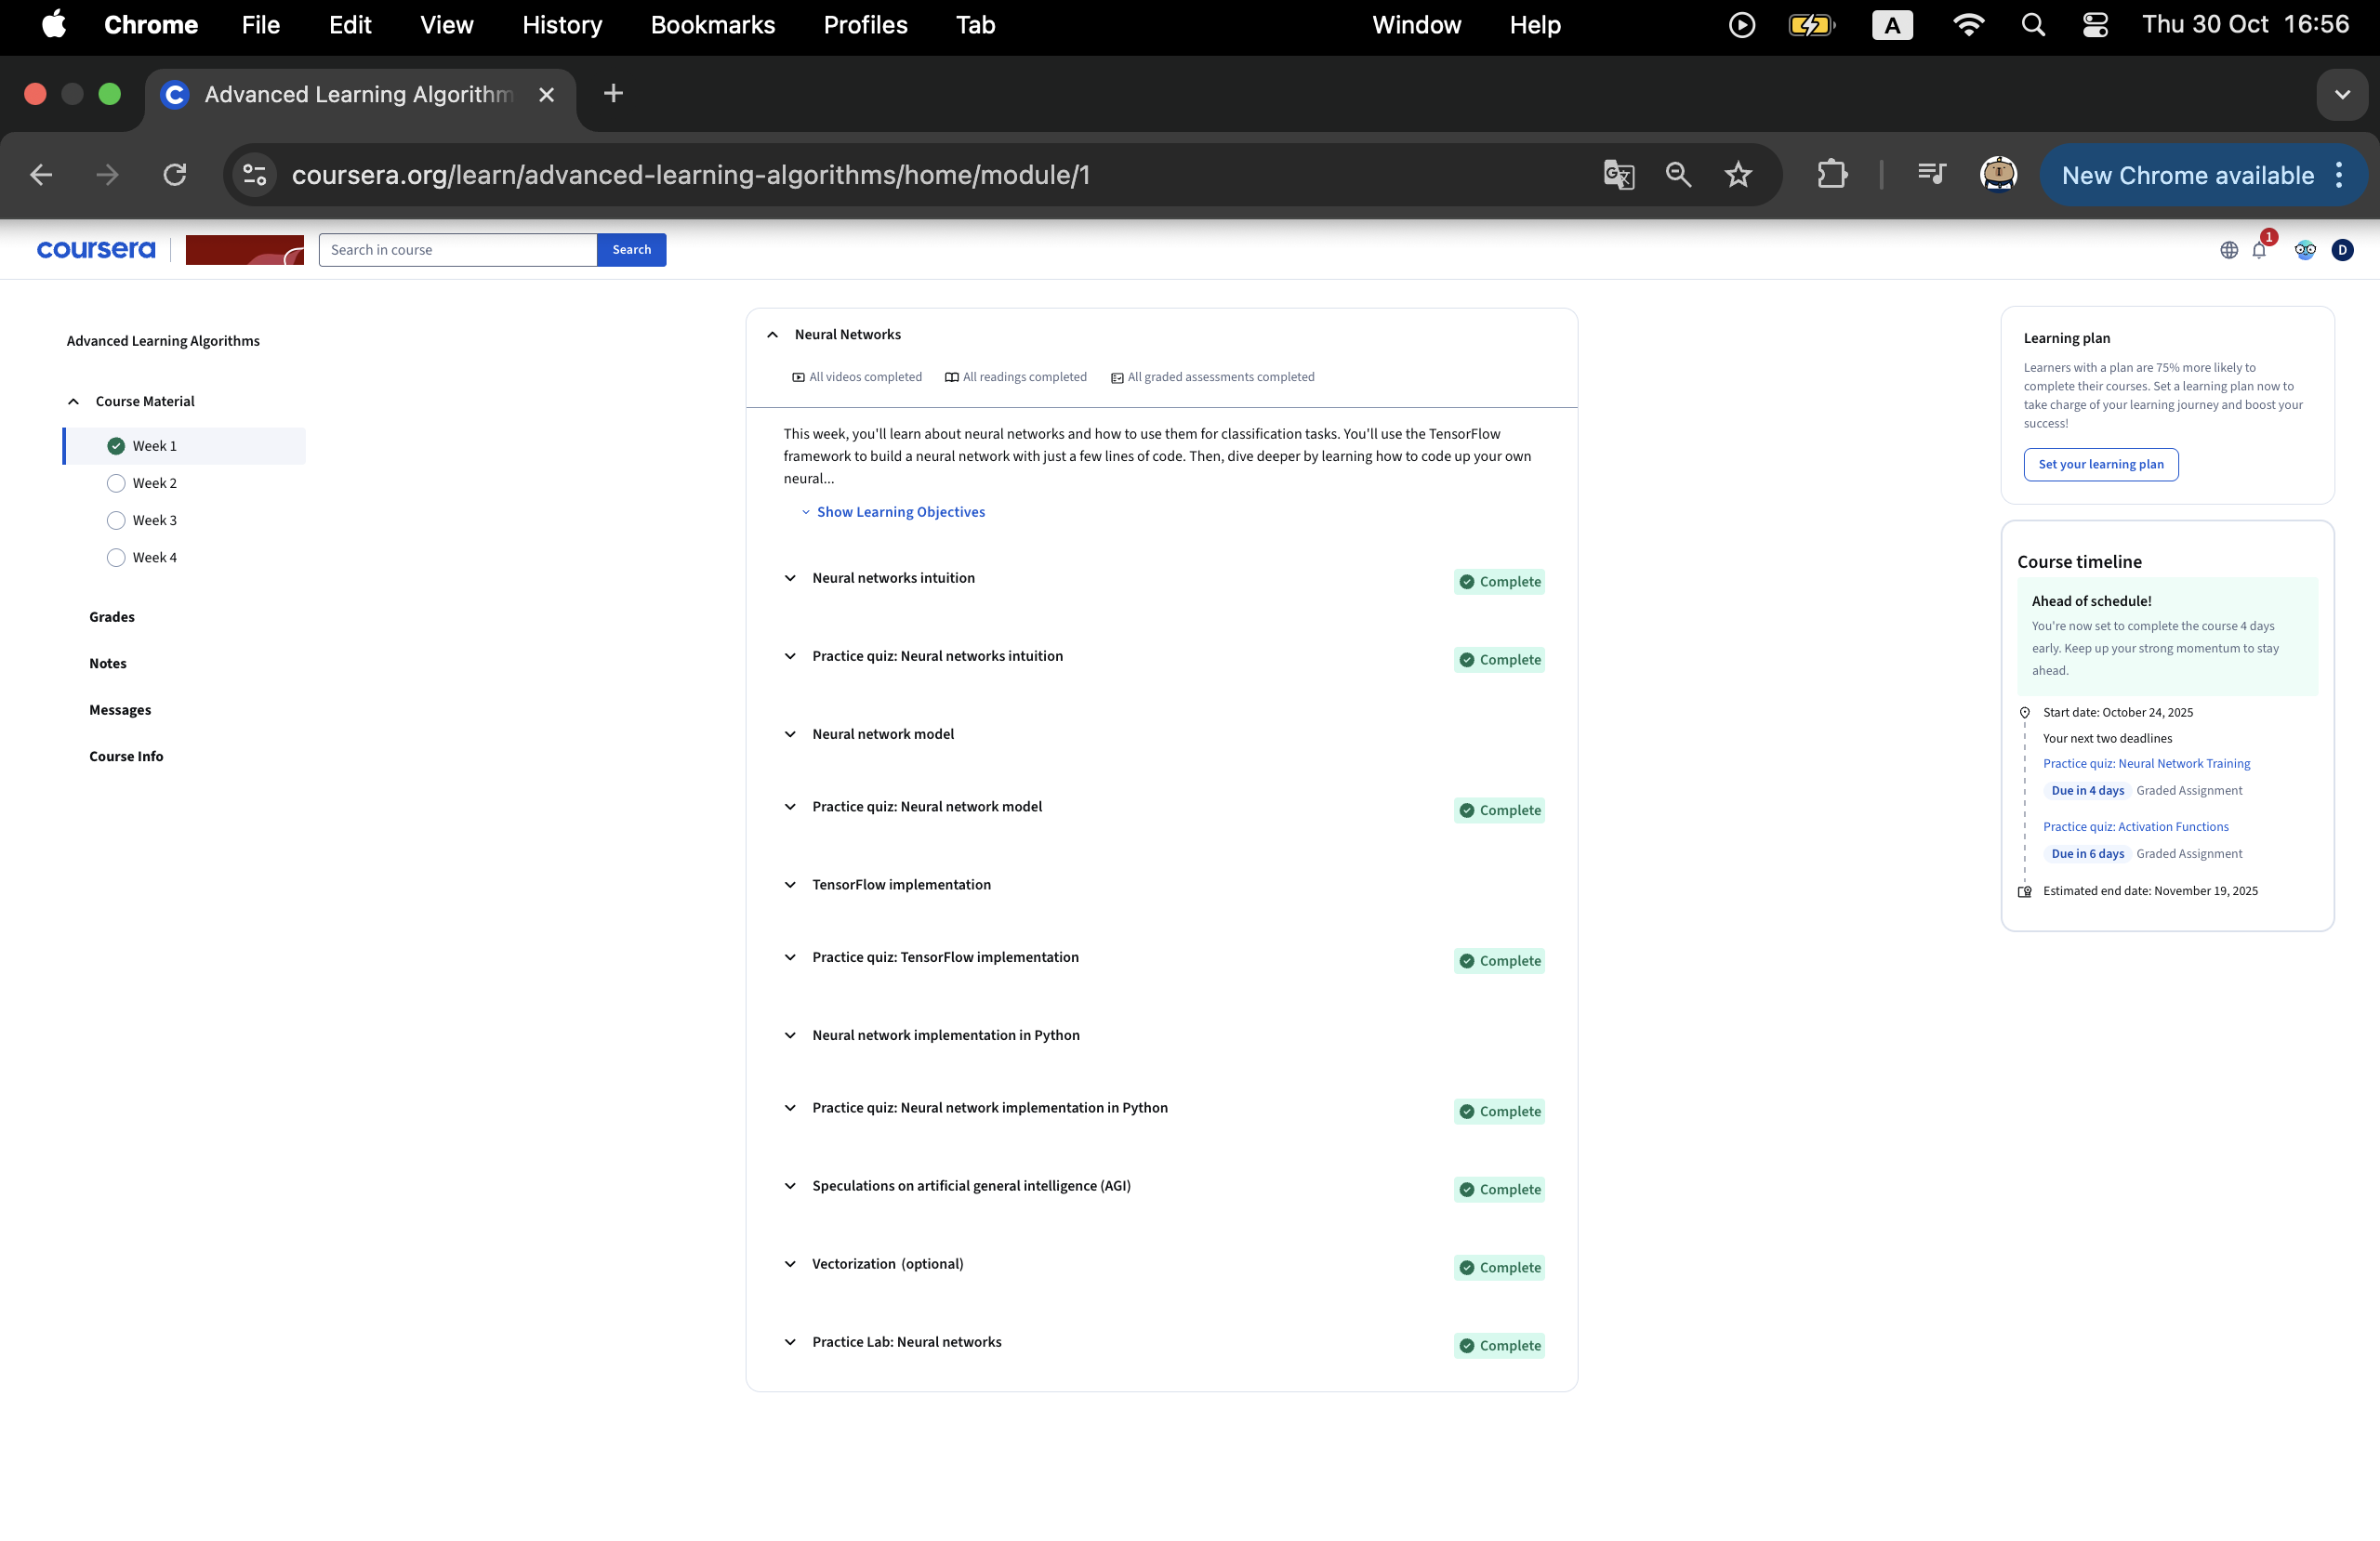
\includegraphics[scale=0.25]{Image/c2_w1.png}
    \caption{Lesson's completed date (30/10/2025)}
\end{figure}

\subsubsection{Graded Assignment Evidence}
\begin{figure}[H]
    \centering
    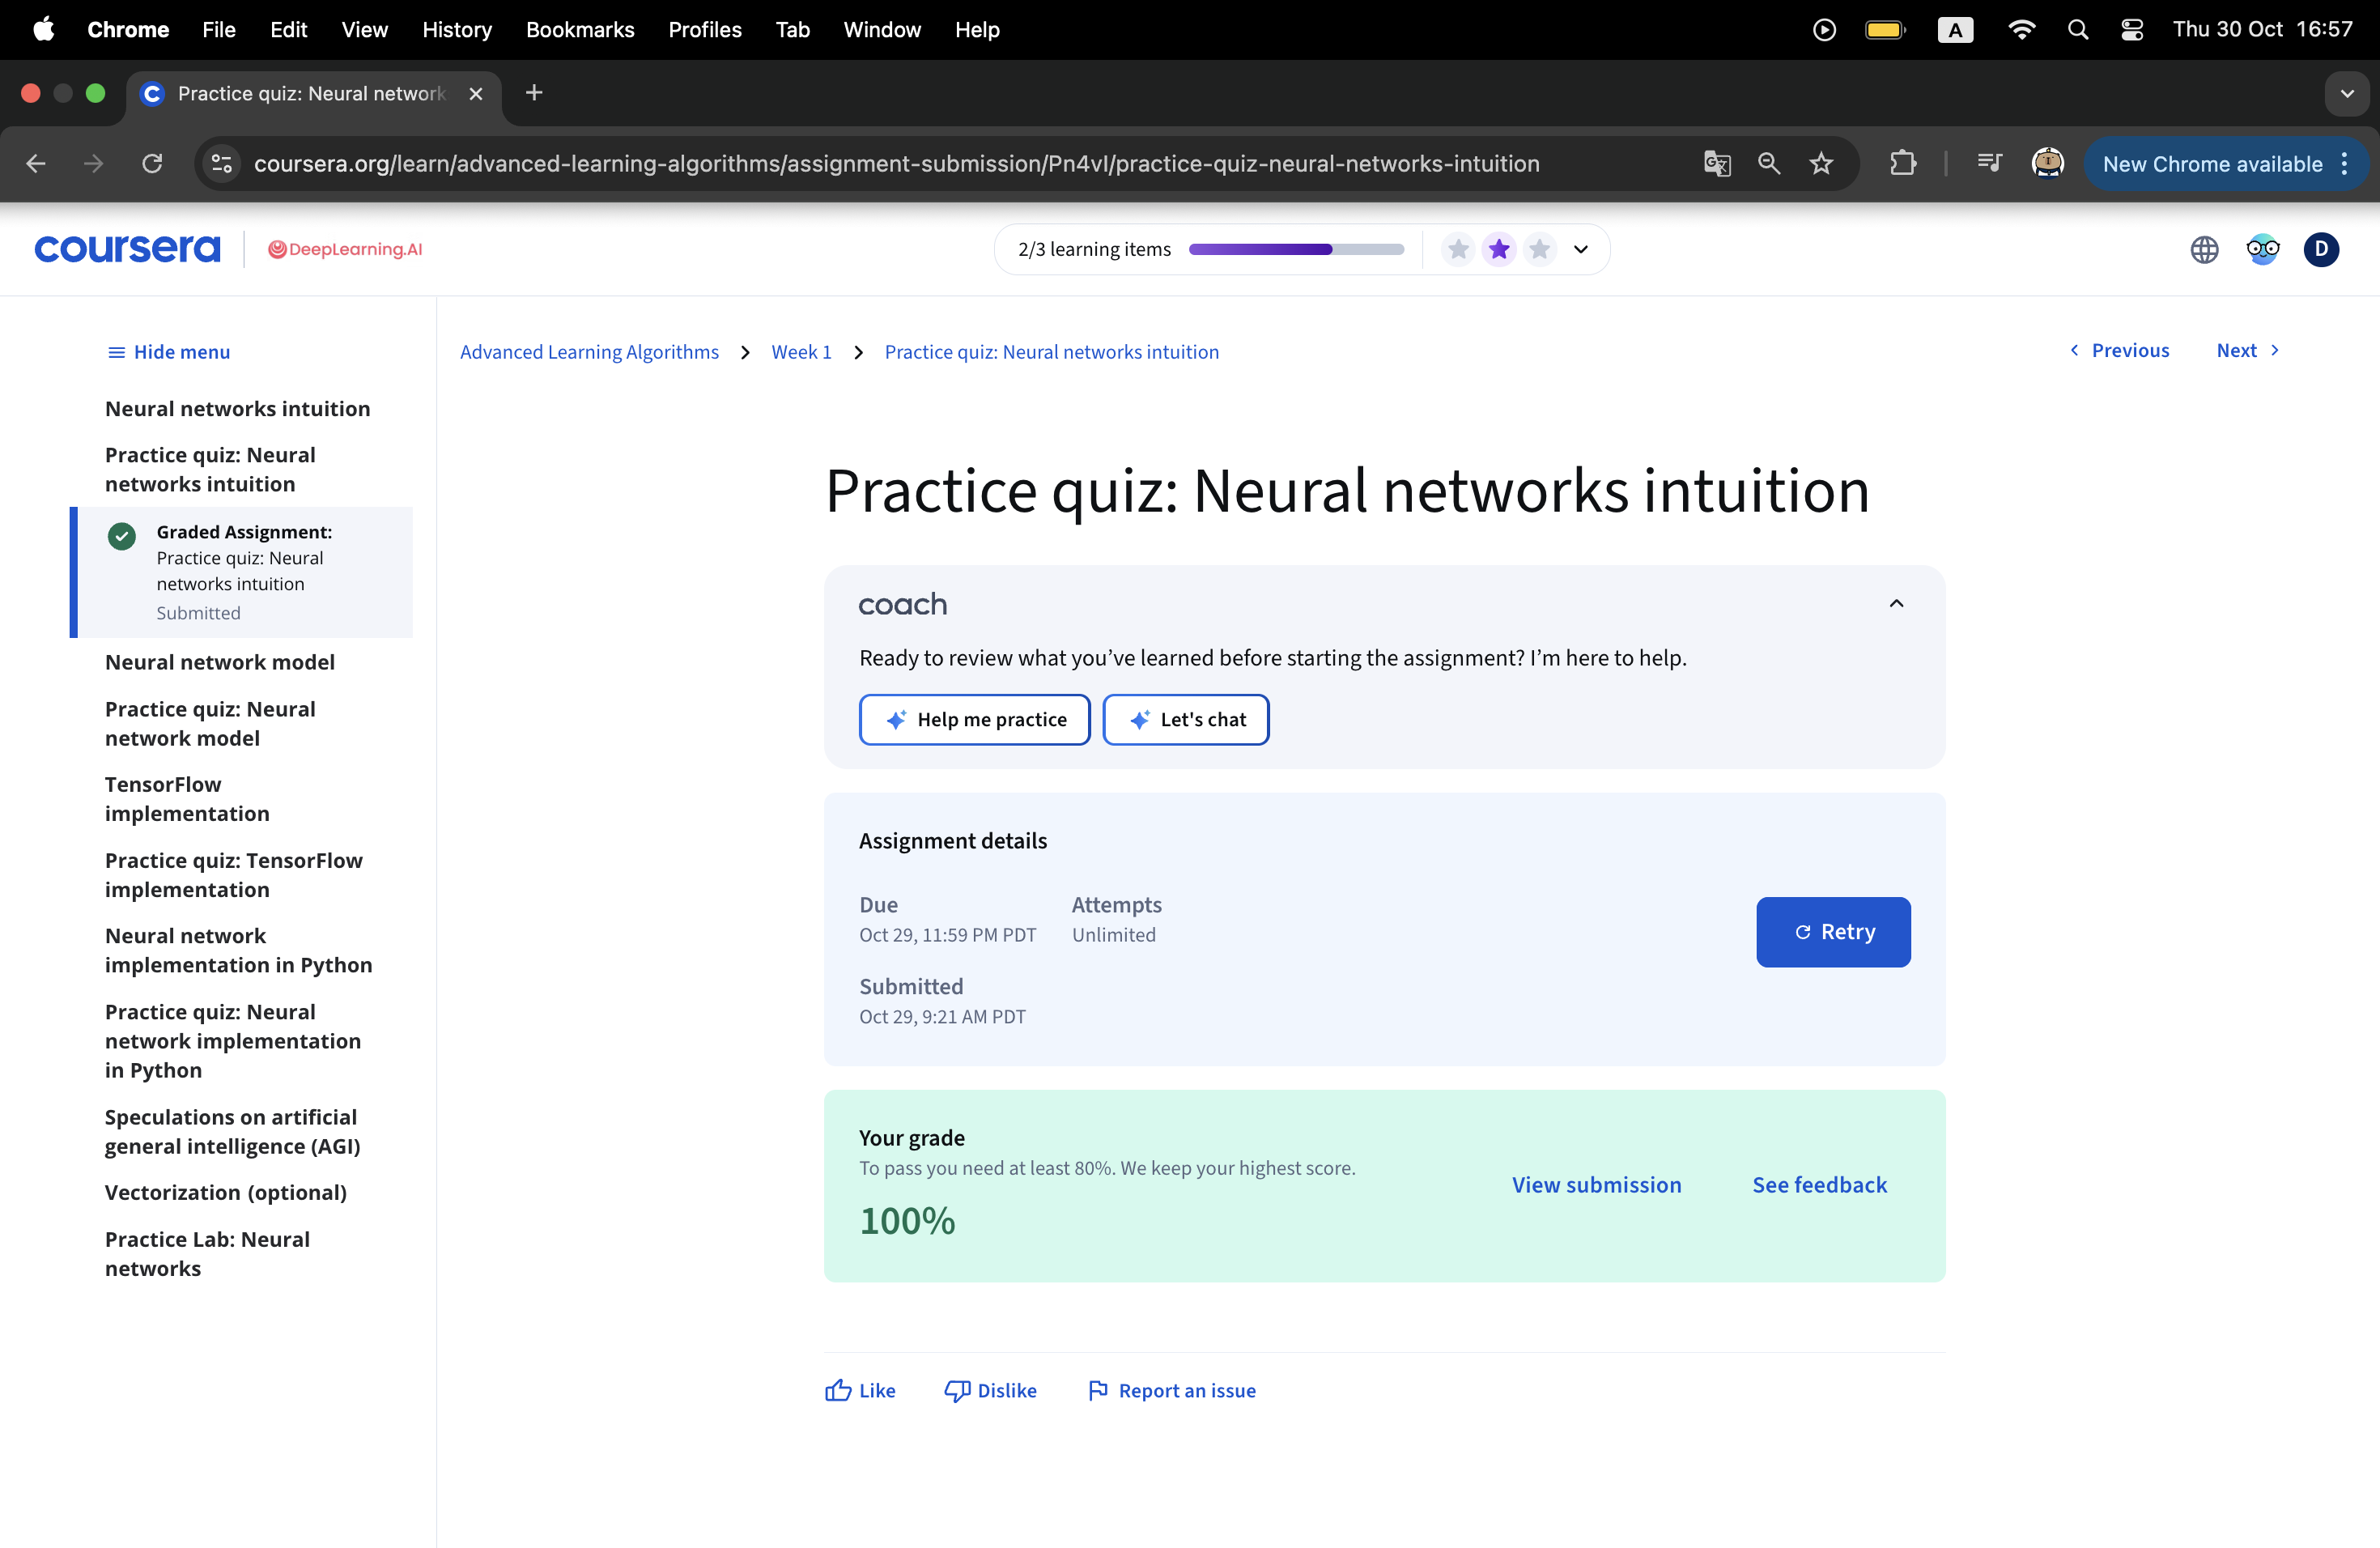
\includegraphics[scale=0.27]{Image/c2_w1_q1.png}
    \caption{Completed Graded Assignment 1 (Neural networks intuition)}
\end{figure}

\begin{figure}[H]
    \centering
    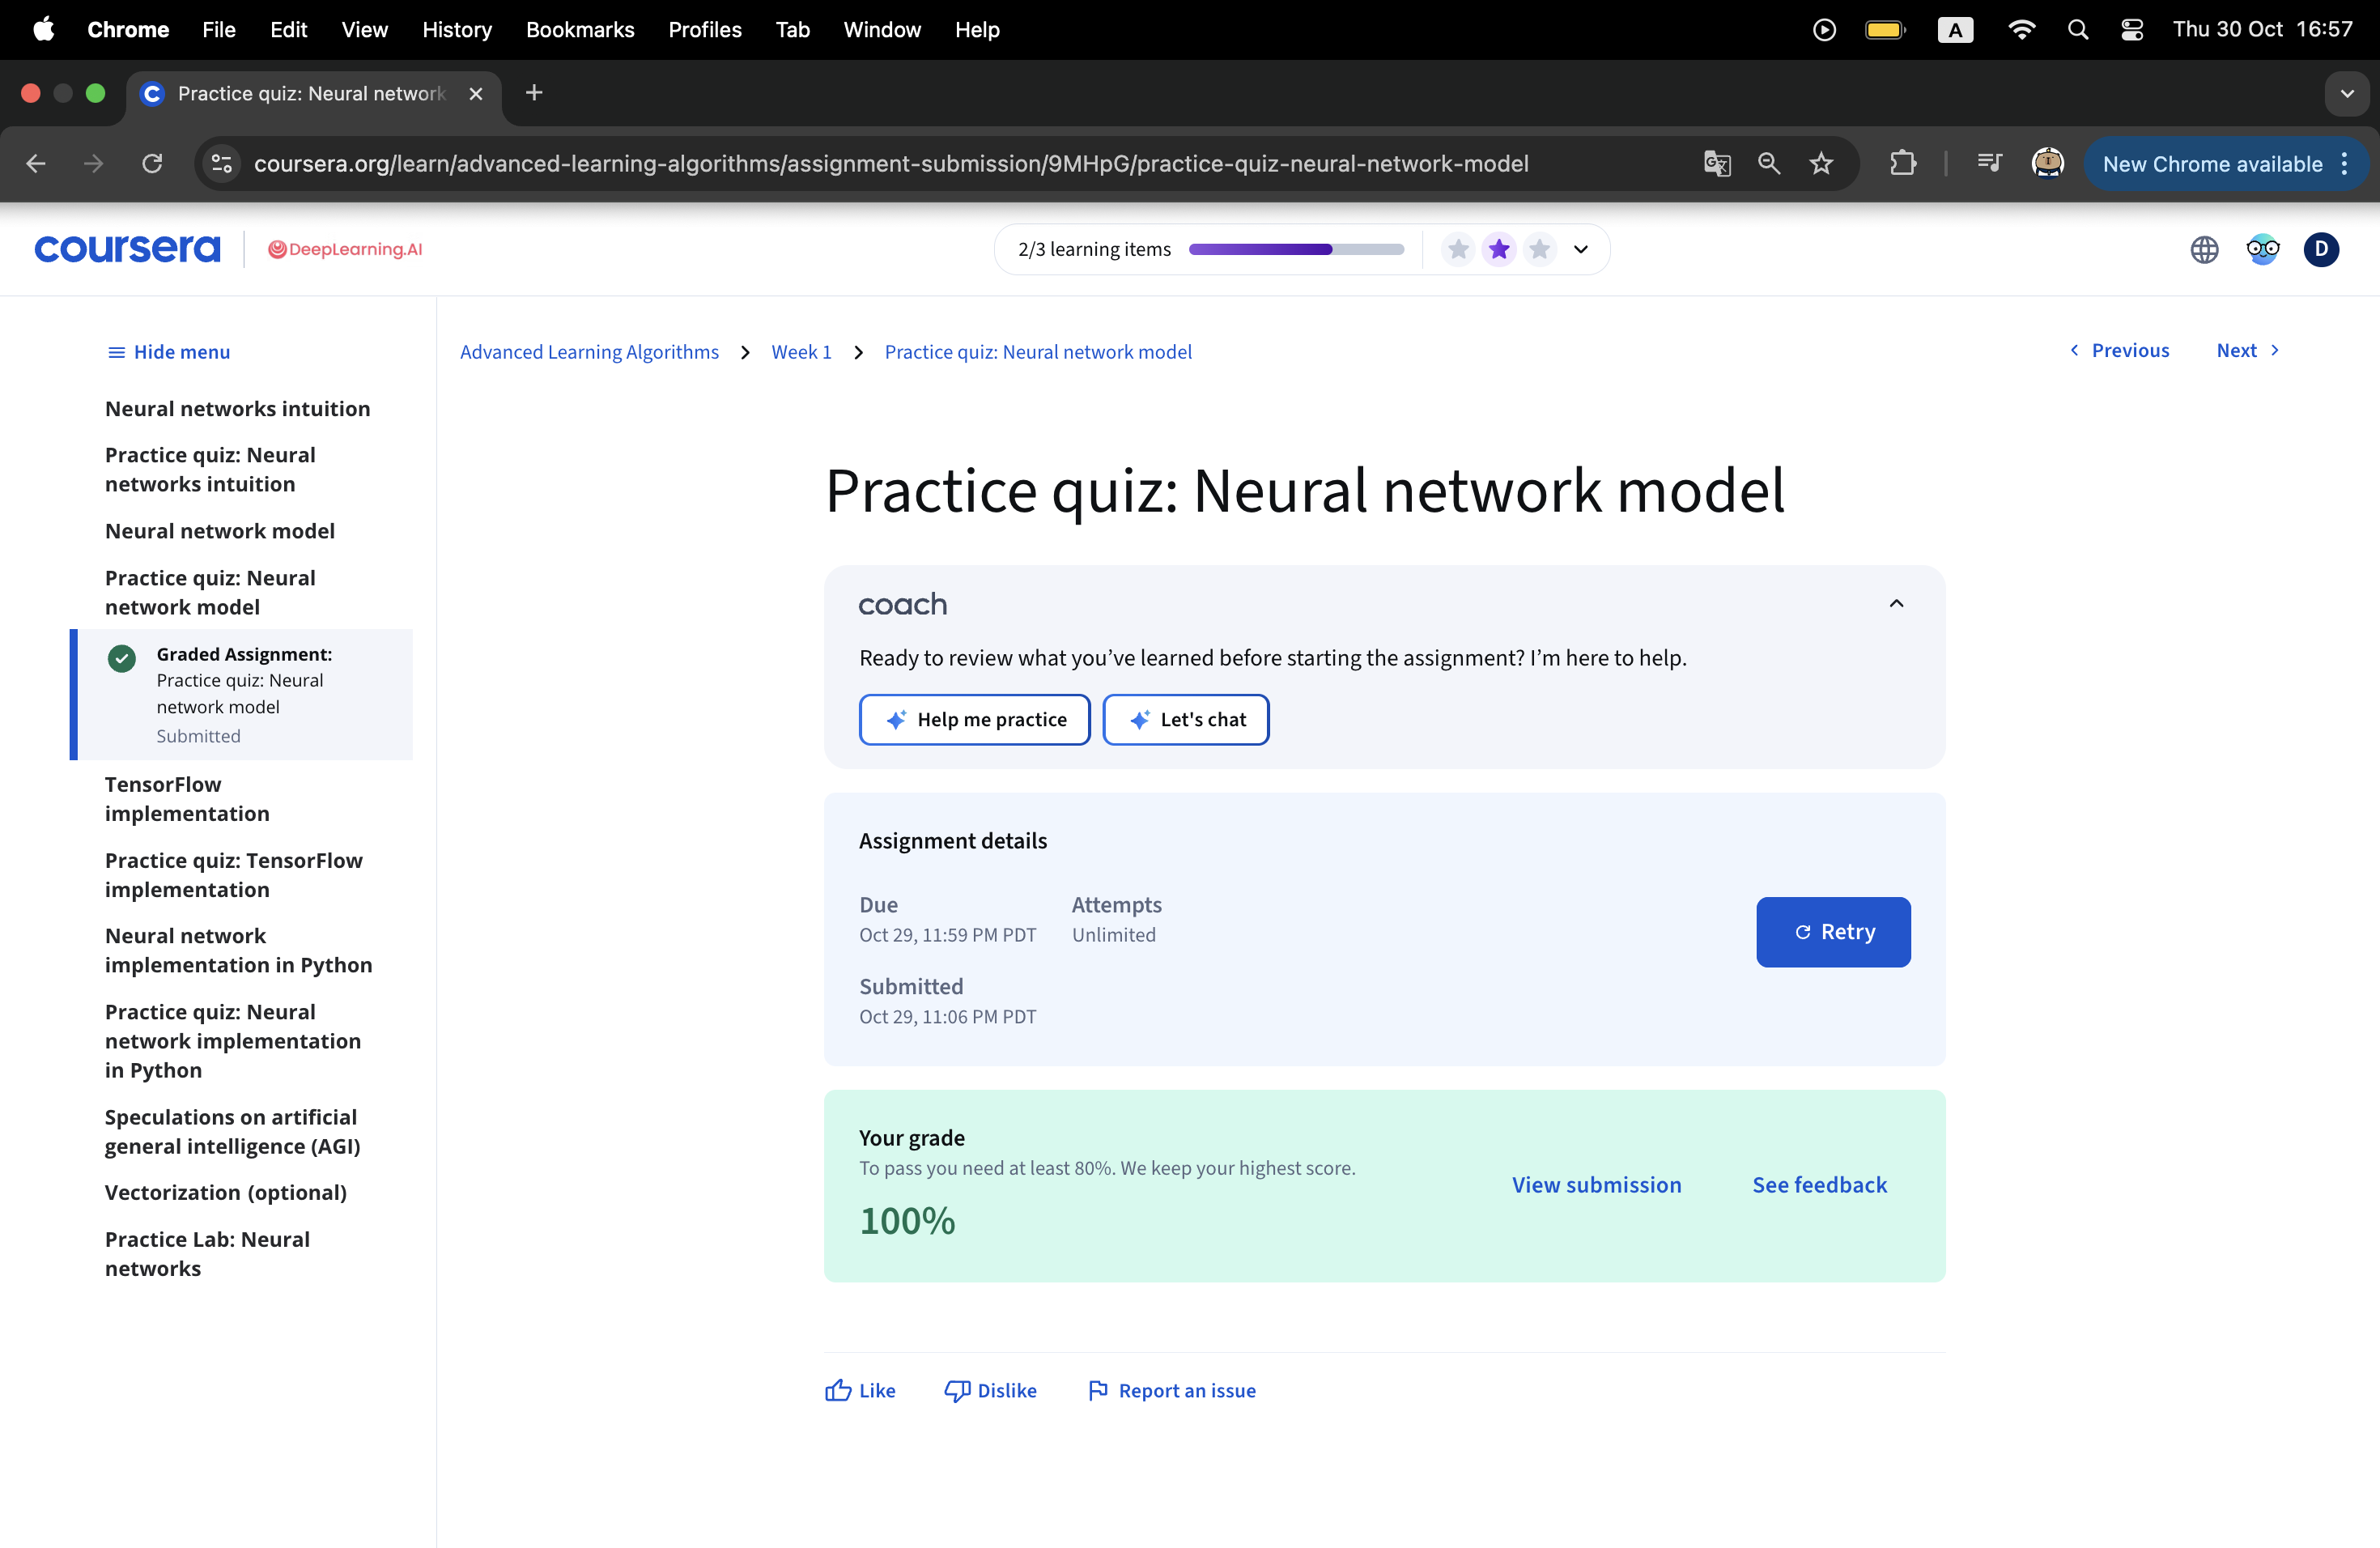
\includegraphics[scale=0.27]{Image/c2_w1_q2.png}
    \caption{Completed Graded Assignment 2 (Neural network model)}
\end{figure}

\begin{figure}[H]
    \centering
    
\includegraphics[scale=0.27]{Image/c2_w1_q3.png}
    \caption{Completed Graded Assignment 3 (TensorFlow implementation)}
\end{figure}

\begin{figure}[H]
    \centering
    
\includegraphics[scale=0.27]{Image/c2_w1_q4.png}
    \caption{Completed Graded Assignment 4 (Neural network implementation in Python)}
\end{figure}

\begin{figure}[H]
    \centering
    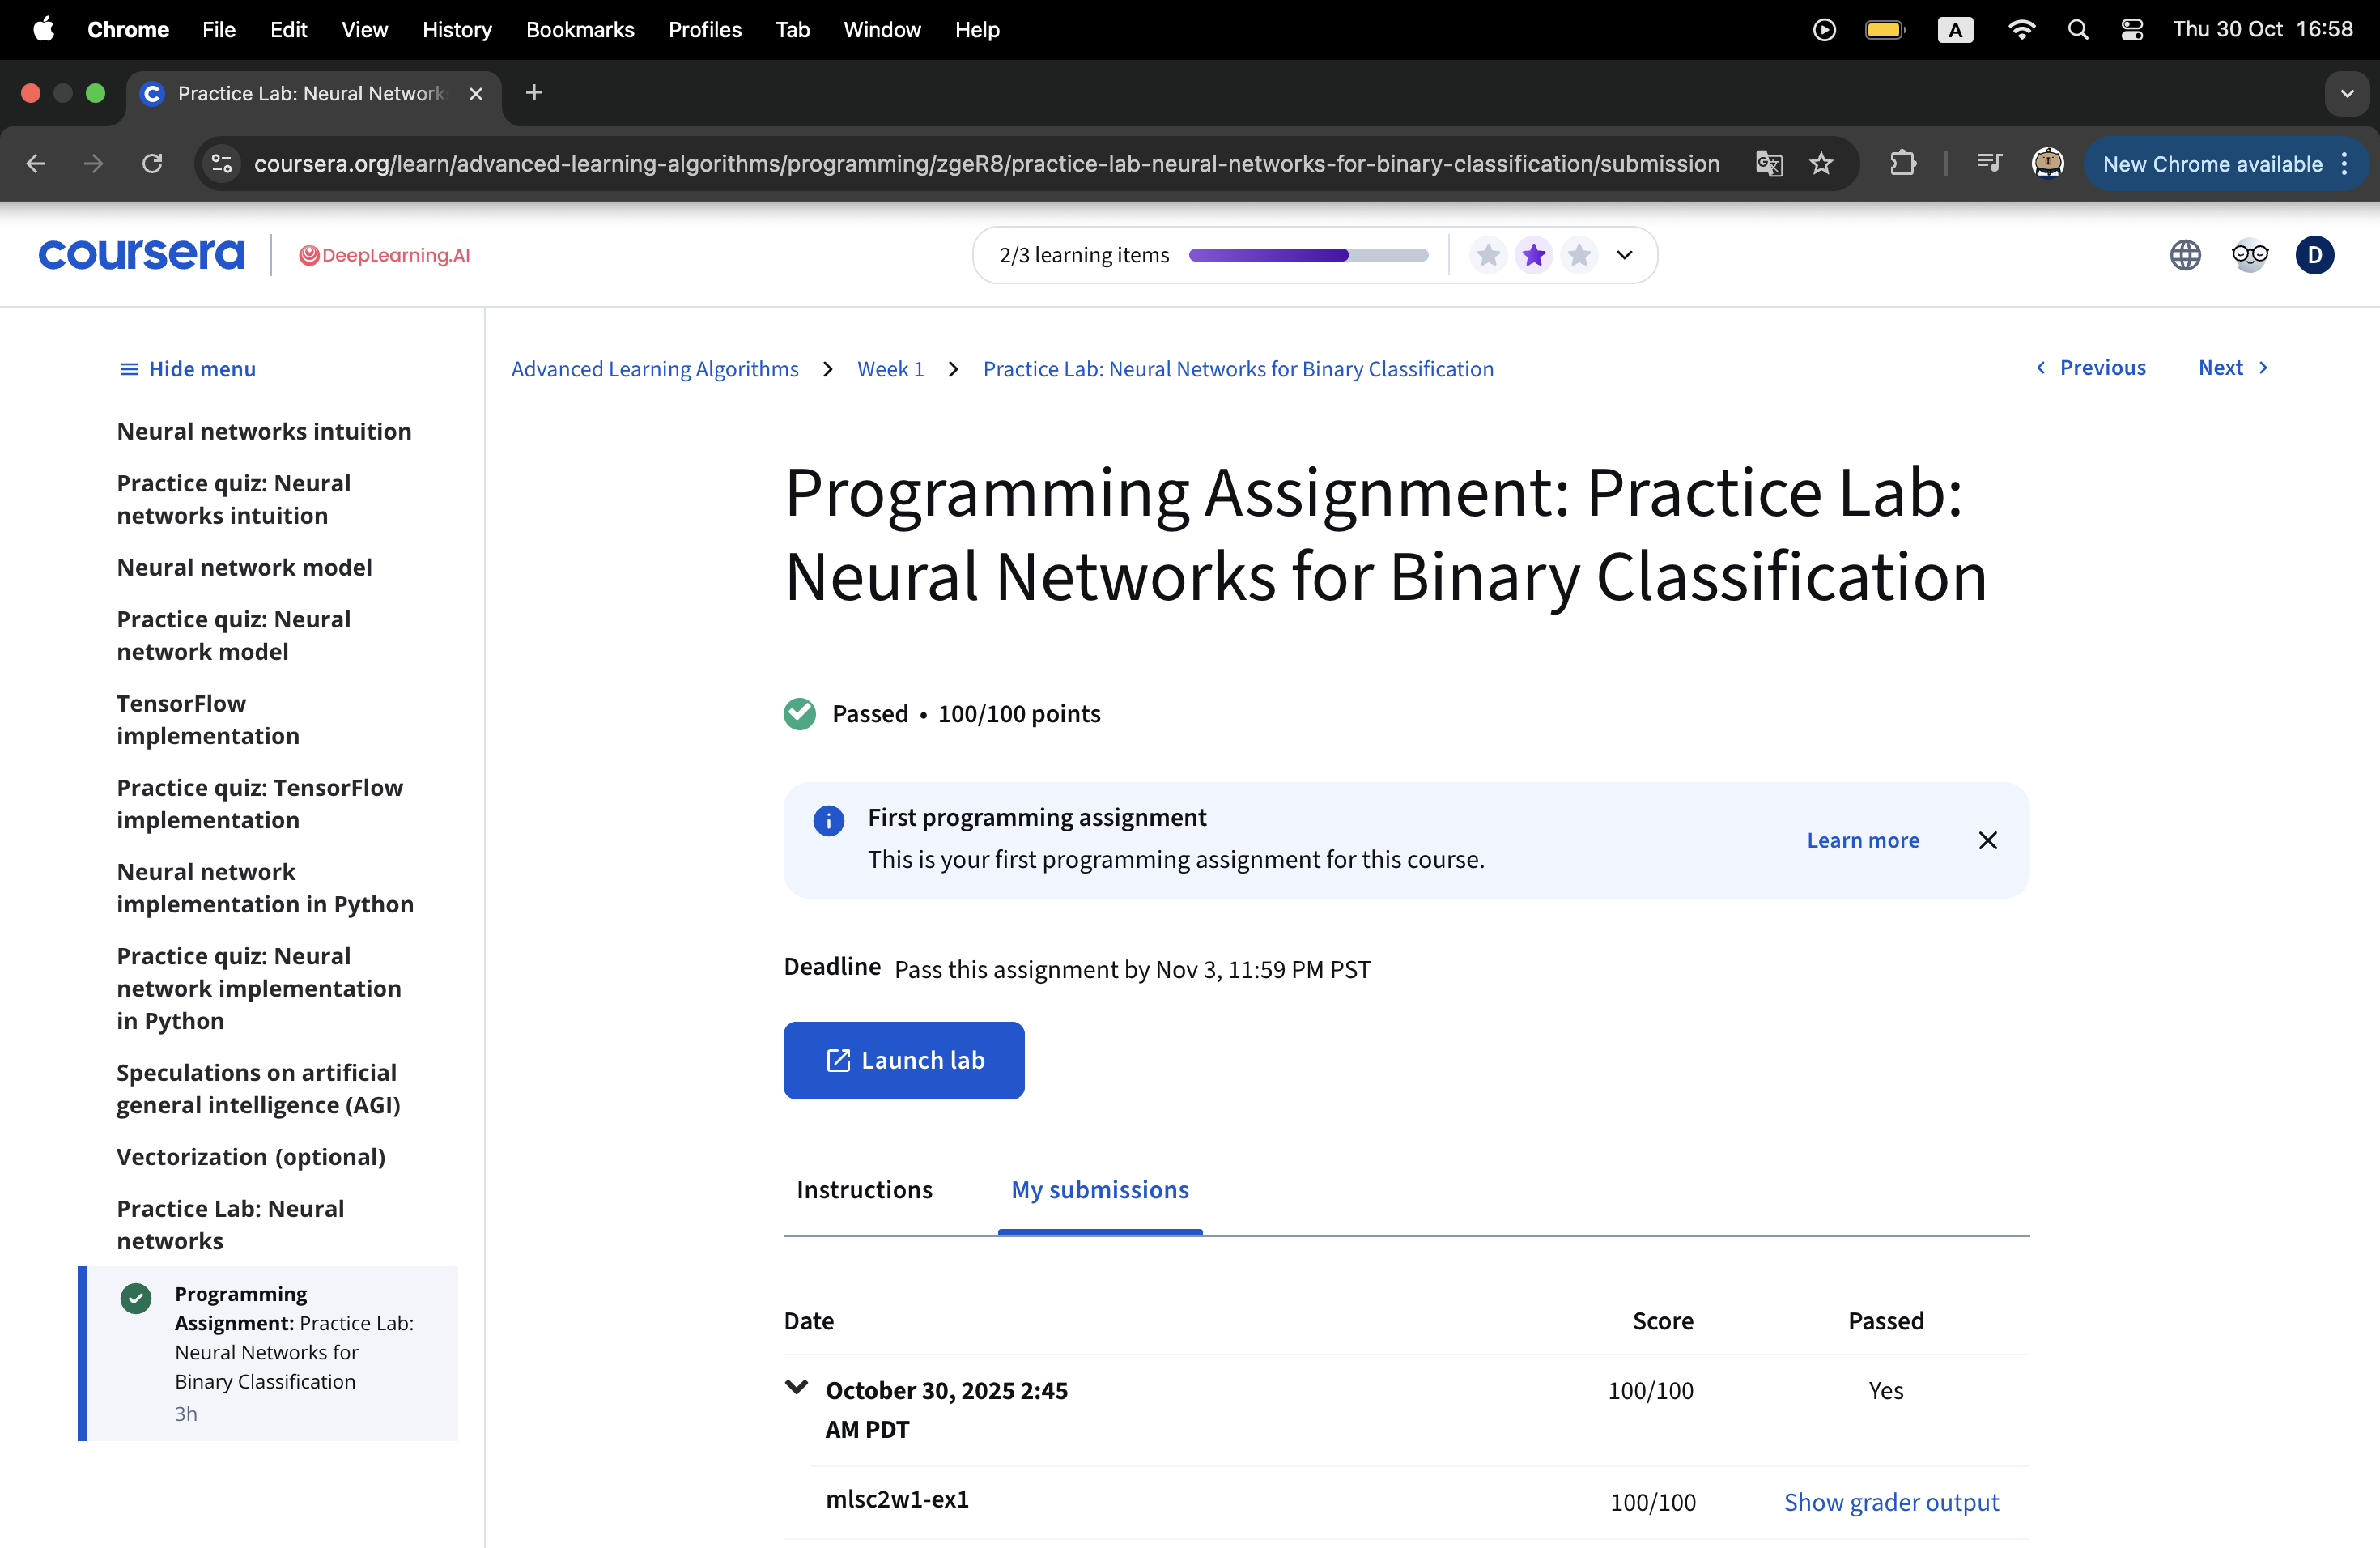
\includegraphics[scale=0.27]{Image/c2_w1_q5.png}
    \caption{Completed Programming Assignment (Neural Networks for Binary Classification)}
\end{figure}

%----------------------------------------
\subsection{Week 2: Neural Network Training}
%----------------------------------------

\subsubsection{Key Insights and Learnings}

This module demystified the "black box" of training, focusing on the mathematical optimization and advanced techniques required for convergence.

\begin{itemize}
    \item \textbf{Backpropagation Algorithm:} Mastered the chain rule application in computation graphs. This algorithm efficiently computes the partial derivatives ($\frac{\partial J}{\partial w}$) of the cost function, guiding the network on how to adjust weights to minimize error.
    
    \item \textbf{Advanced Optimization:} 
    \begin{itemize}
        \item Moved beyond standard Gradient Descent to \textbf{Adam (Adaptive Moment Estimation)}.
        \item \textbf{Adam} adjusts learning rates individually for each parameter, resulting in faster convergence and better handling of local optima compared to standard SGD.
    \end{itemize}

    \item \textbf{Handling Overfitting (Regularization):} Implemented strategies to improve model generalization:
    \begin{itemize}
        \item \textbf{L2 Regularization:} Penalizing large weights in the cost function.
        \item \textbf{Dropout:} Randomly deactivating neurons during training to prevent over-reliance on specific features.
    \end{itemize}
\end{itemize}

\subsubsection{Learning Evidence}
\begin{figure}[H]
    \centering
    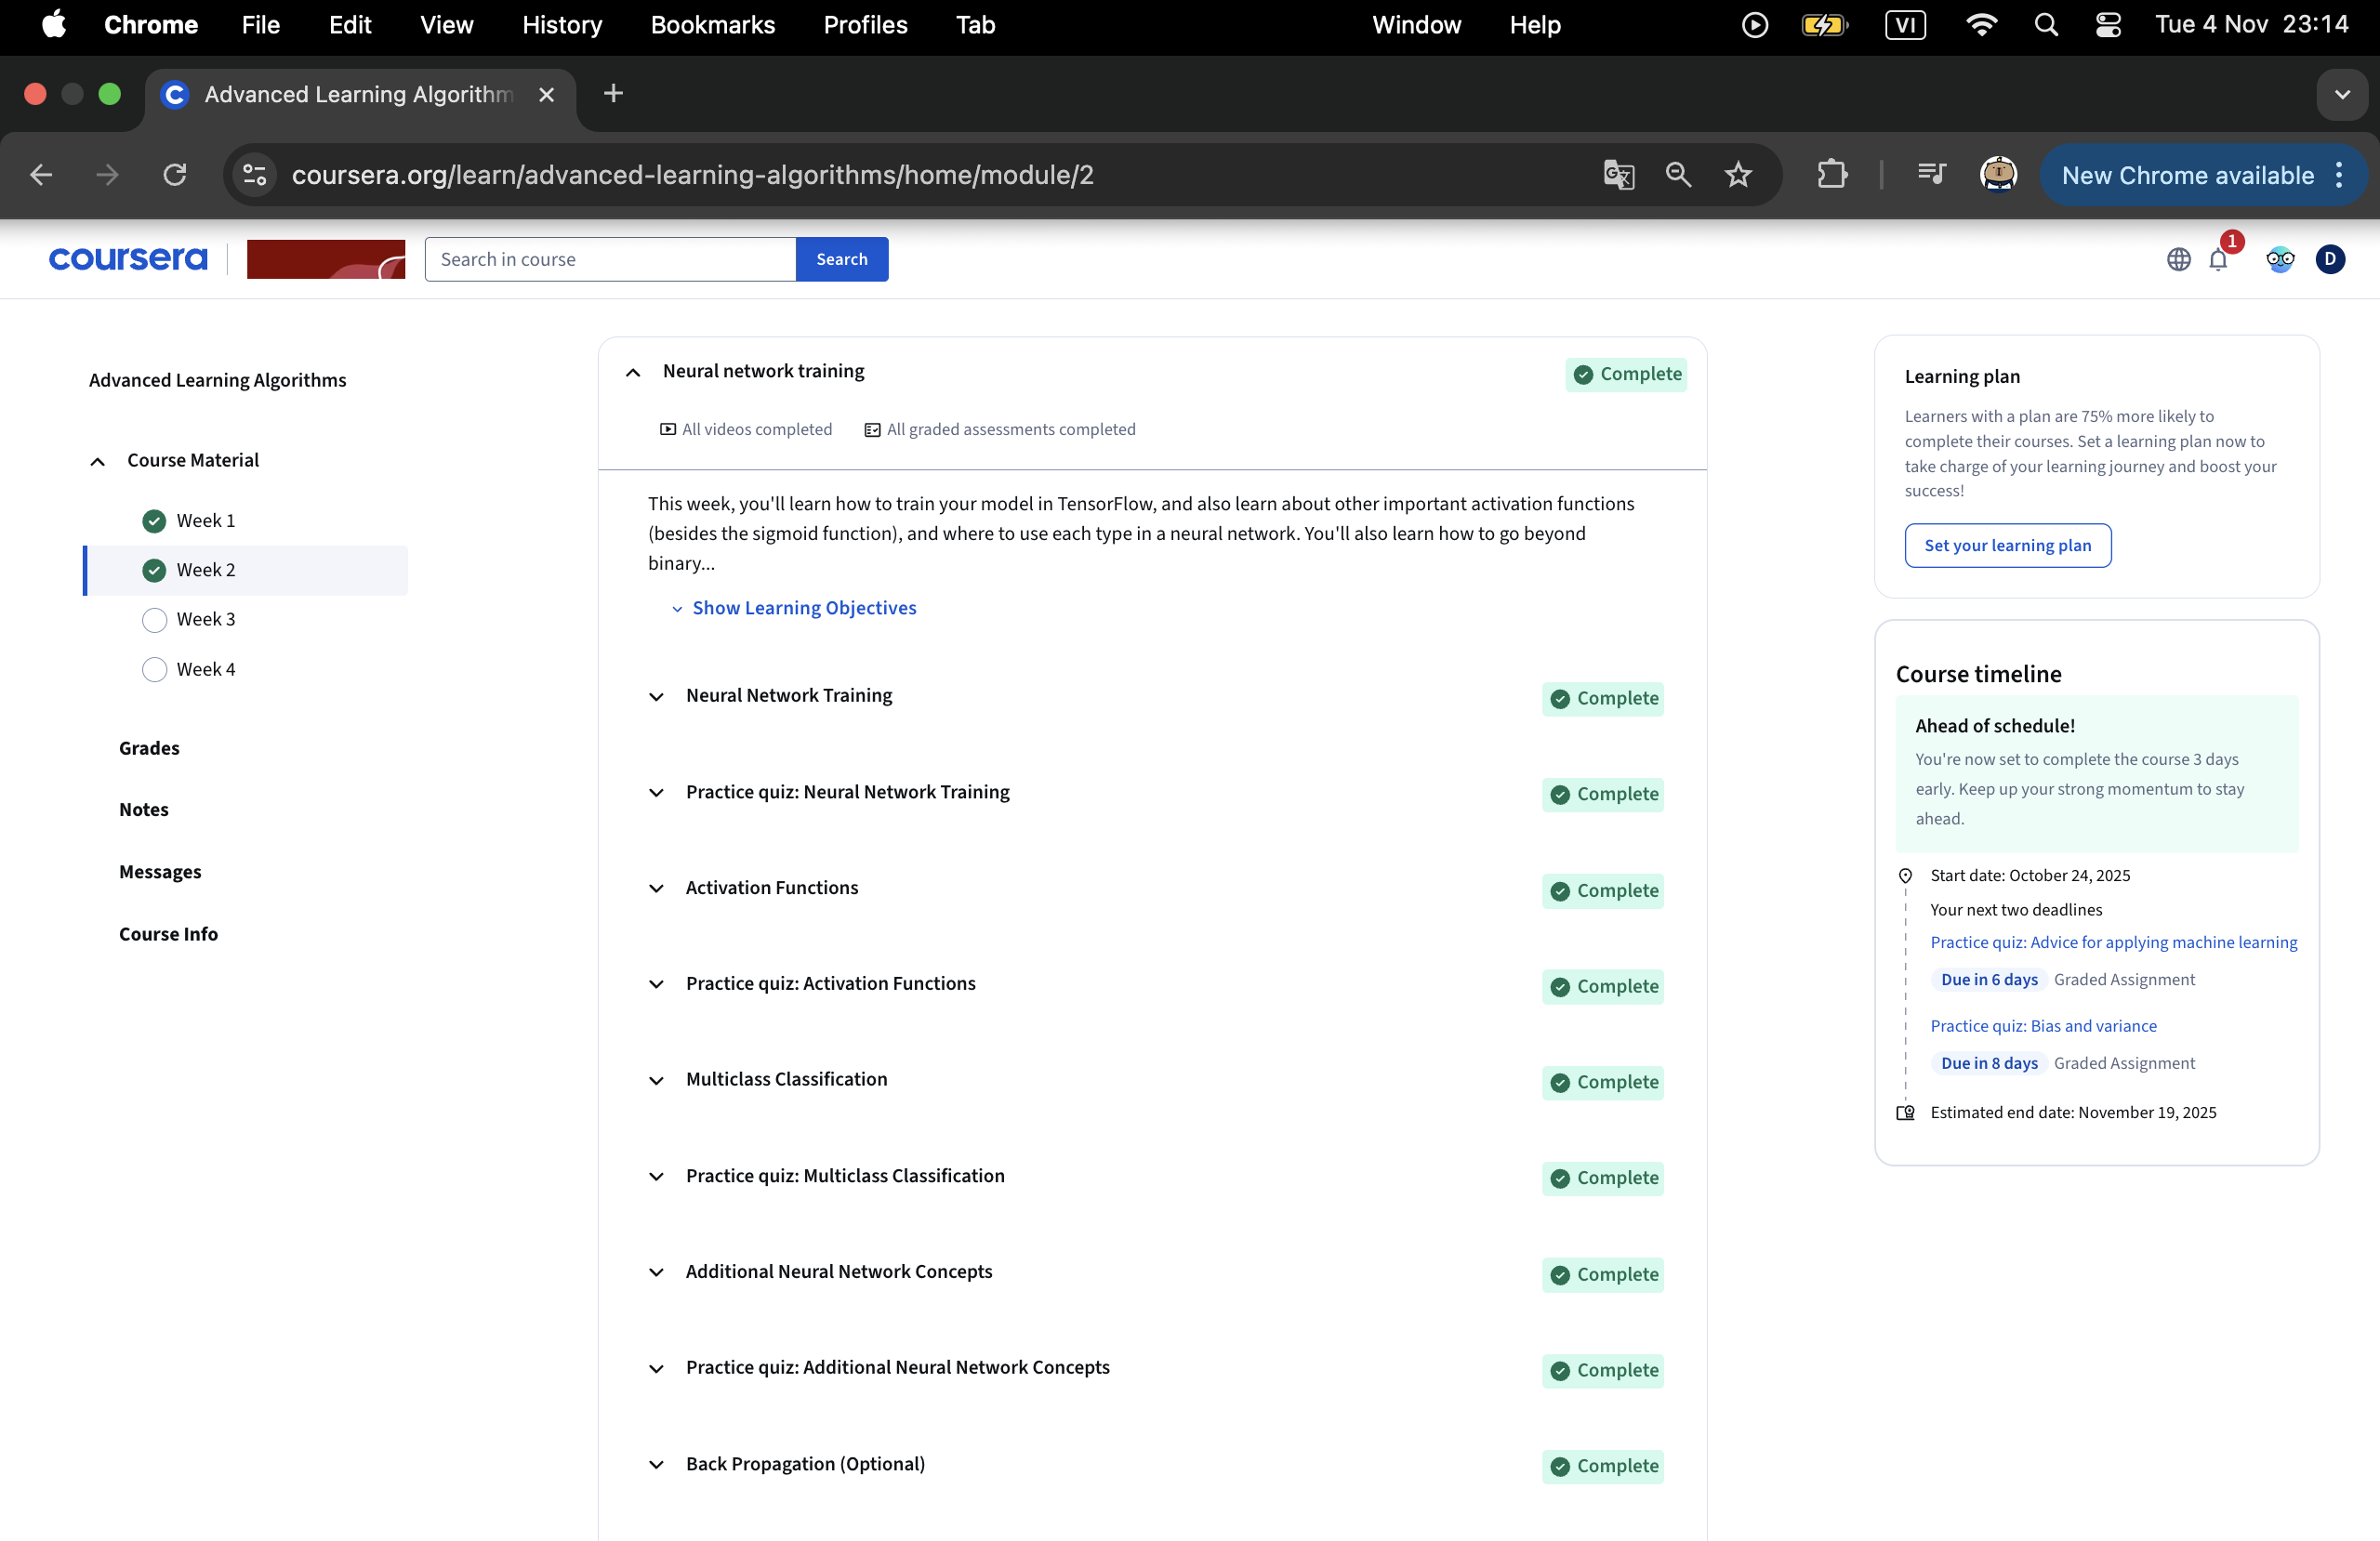
\includegraphics[scale=0.27]{Image/c2_w2.png}
    \caption{Lesson's completed date (04/11/2025)}
\end{figure}

\subsubsection{Graded Assignment Evidence}
\begin{figure}[H]
    \centering
    
\includegraphics[scale=0.25]{Image/c2_w2_q1.png}
    \caption{Completed Graded Assignment 1 (Neural Network Training)}
\end{figure}

\begin{figure}[H]
    \centering
    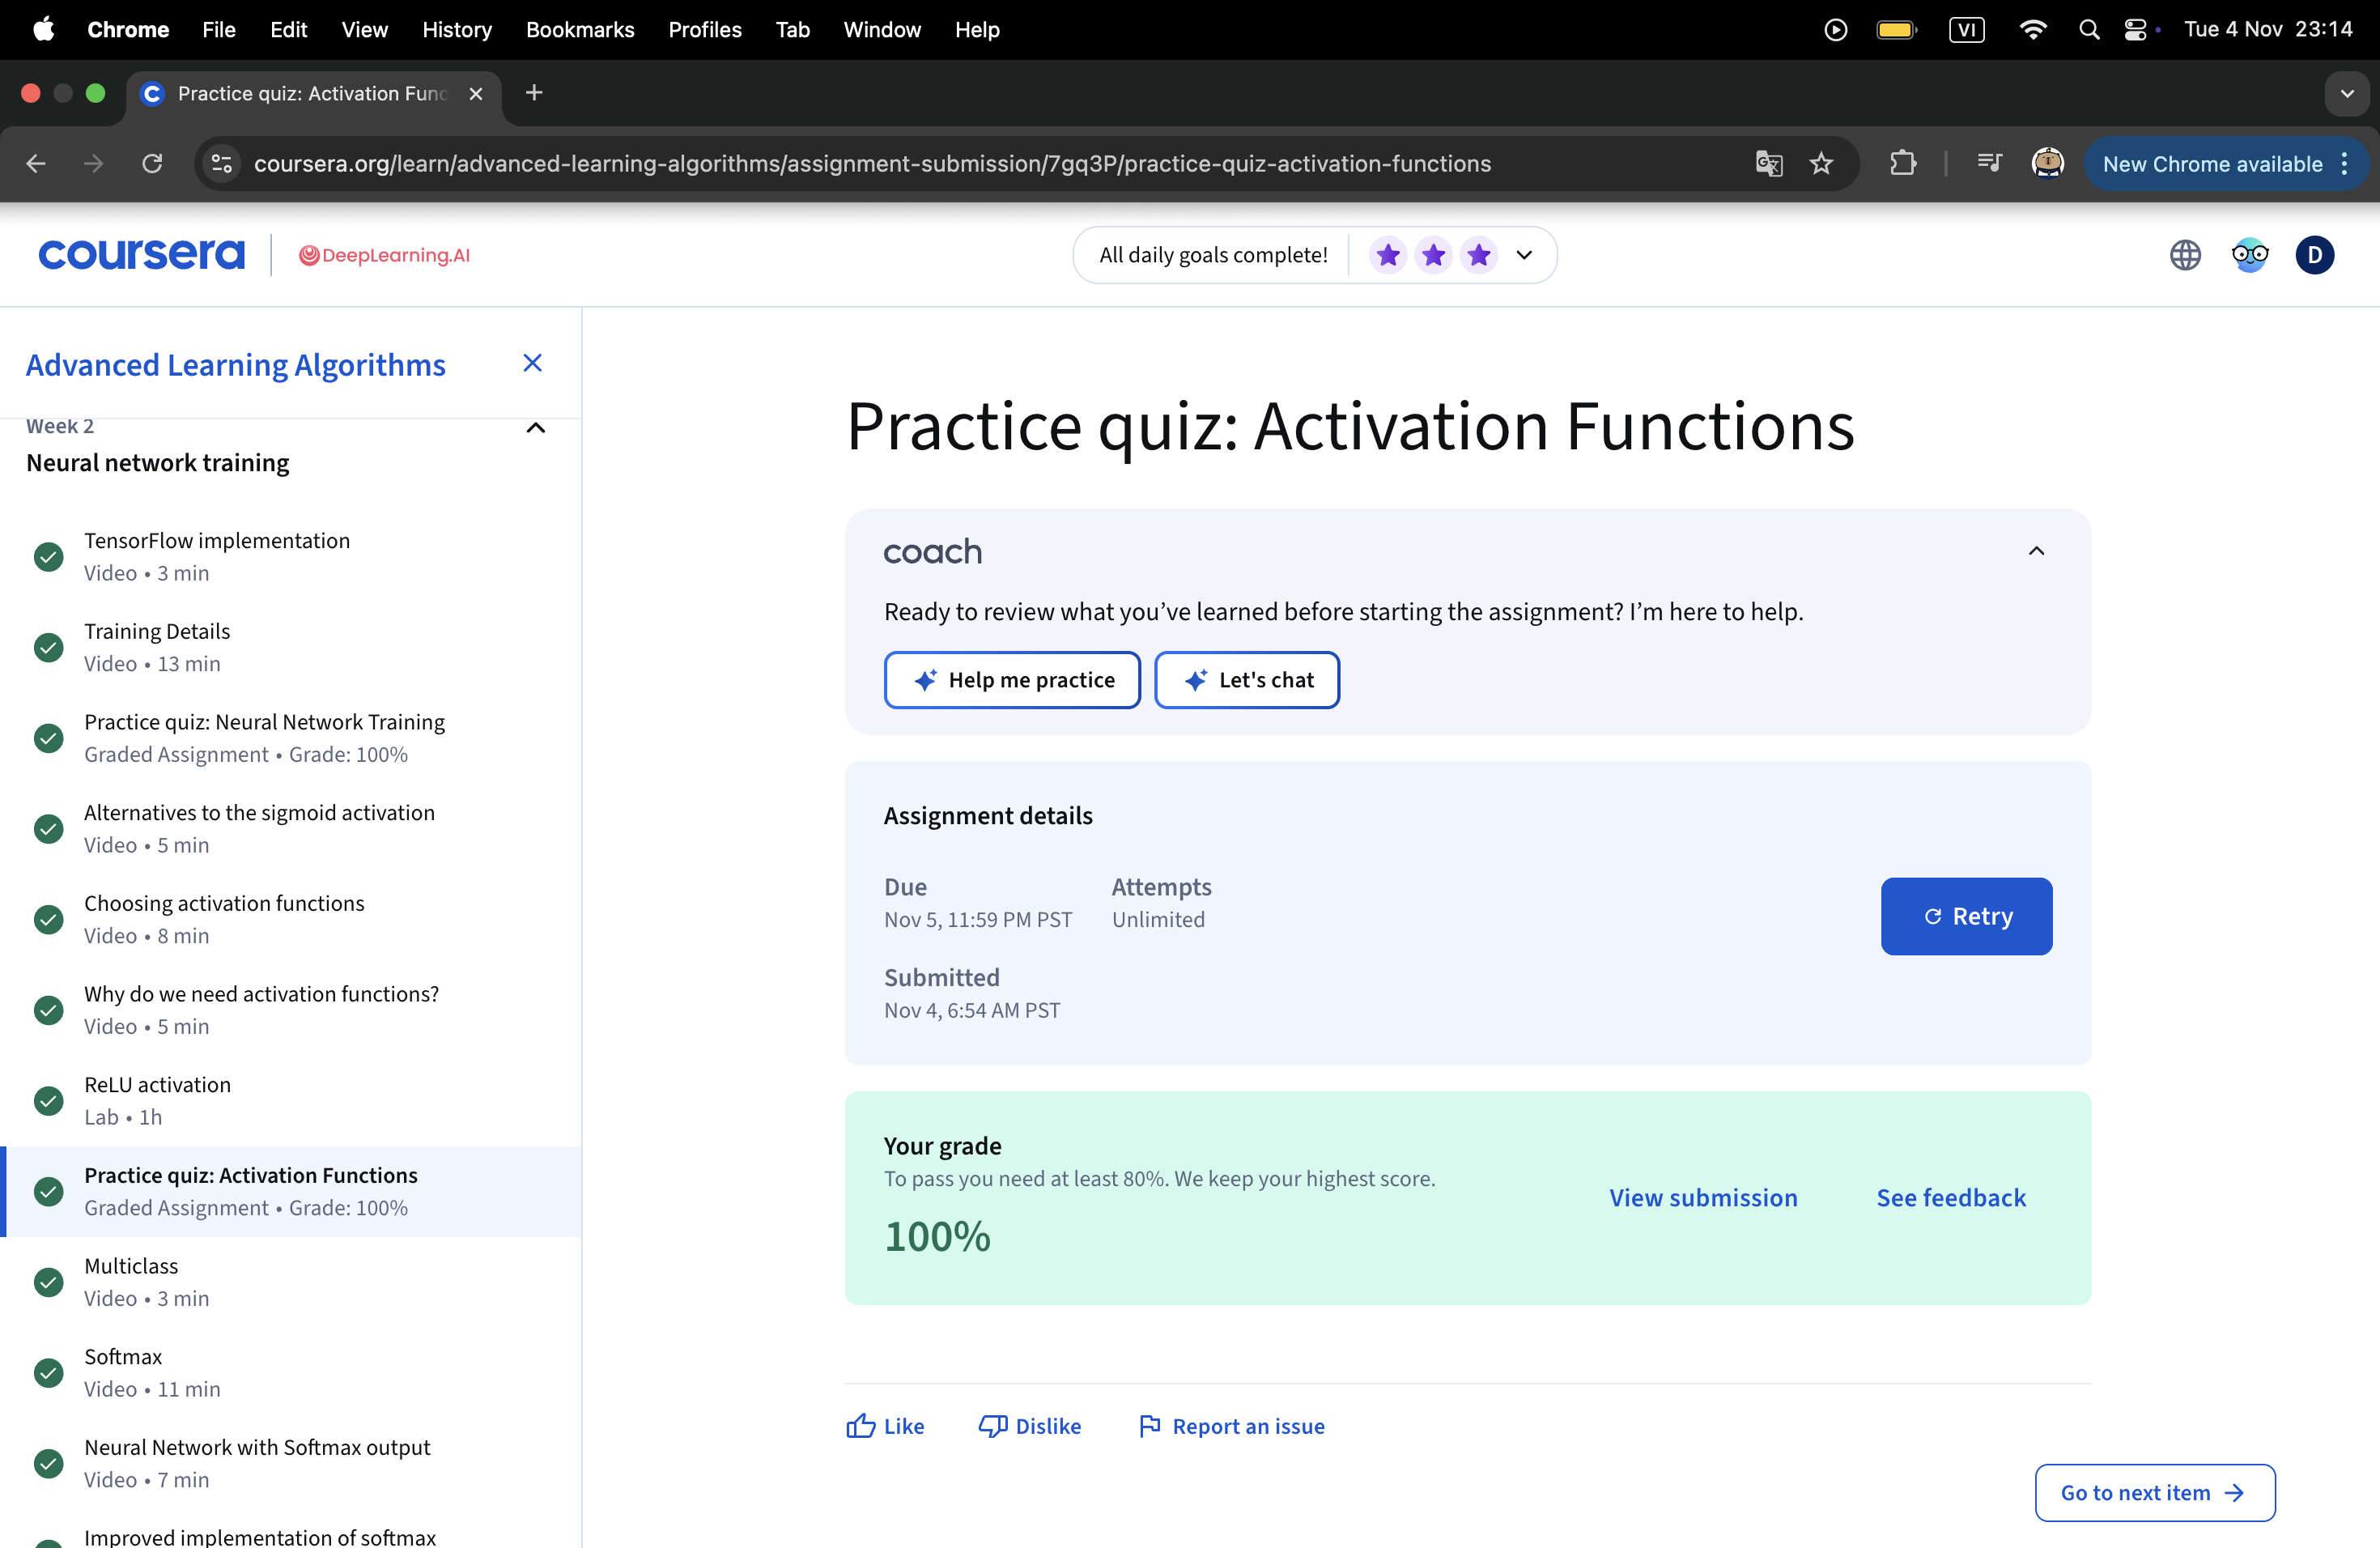
\includegraphics[scale=0.27]{Image/c2_w2_q2.png}
    \caption{Completed Graded Assignment 2 (Activation Functions)}
\end{figure}

\begin{figure}[H]
    \centering
    
\includegraphics[scale=0.27]{Image/c2_w2_q3.png}
    \caption{Completed Graded Assignment 3 (Multiclass Classification)}
\end{figure}

\begin{figure}[H]
    \centering
    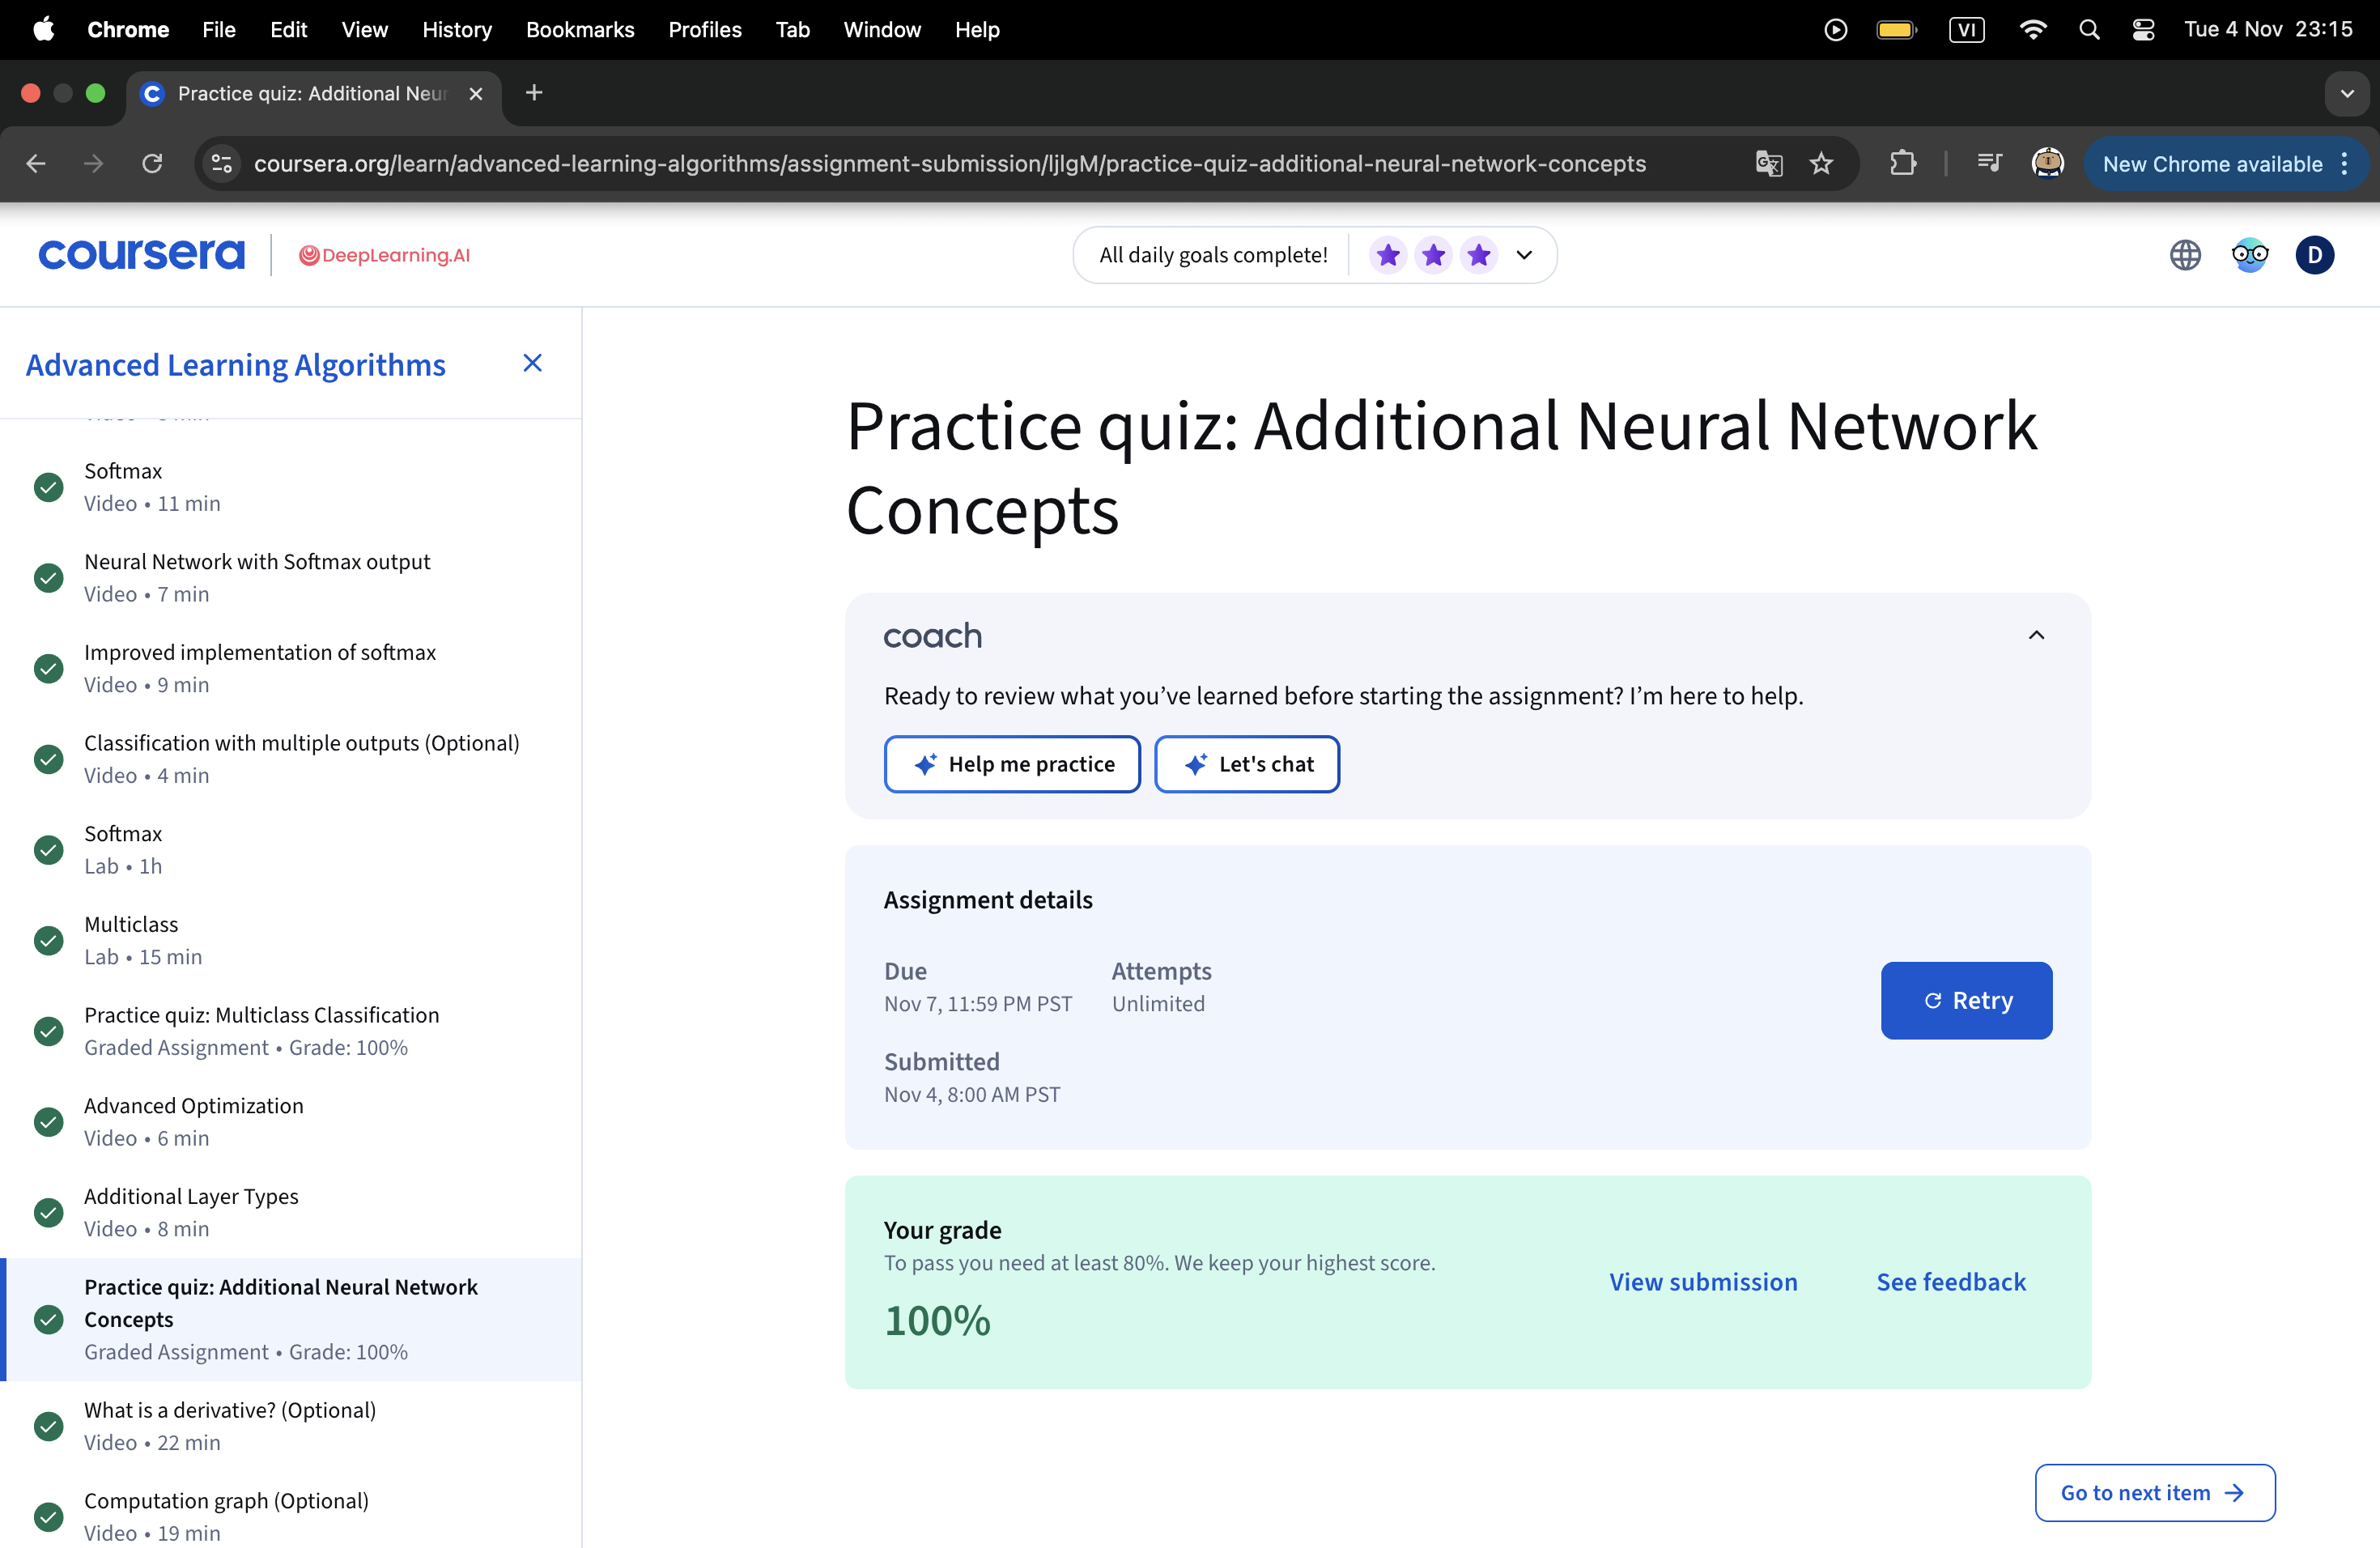
\includegraphics[scale=0.27]{Image/c2_w2_q4.png}
    \caption{Completed Graded Assignment 4 (Additional Neural Network Concepts)}
\end{figure}

\begin{figure}[H]
    \centering
    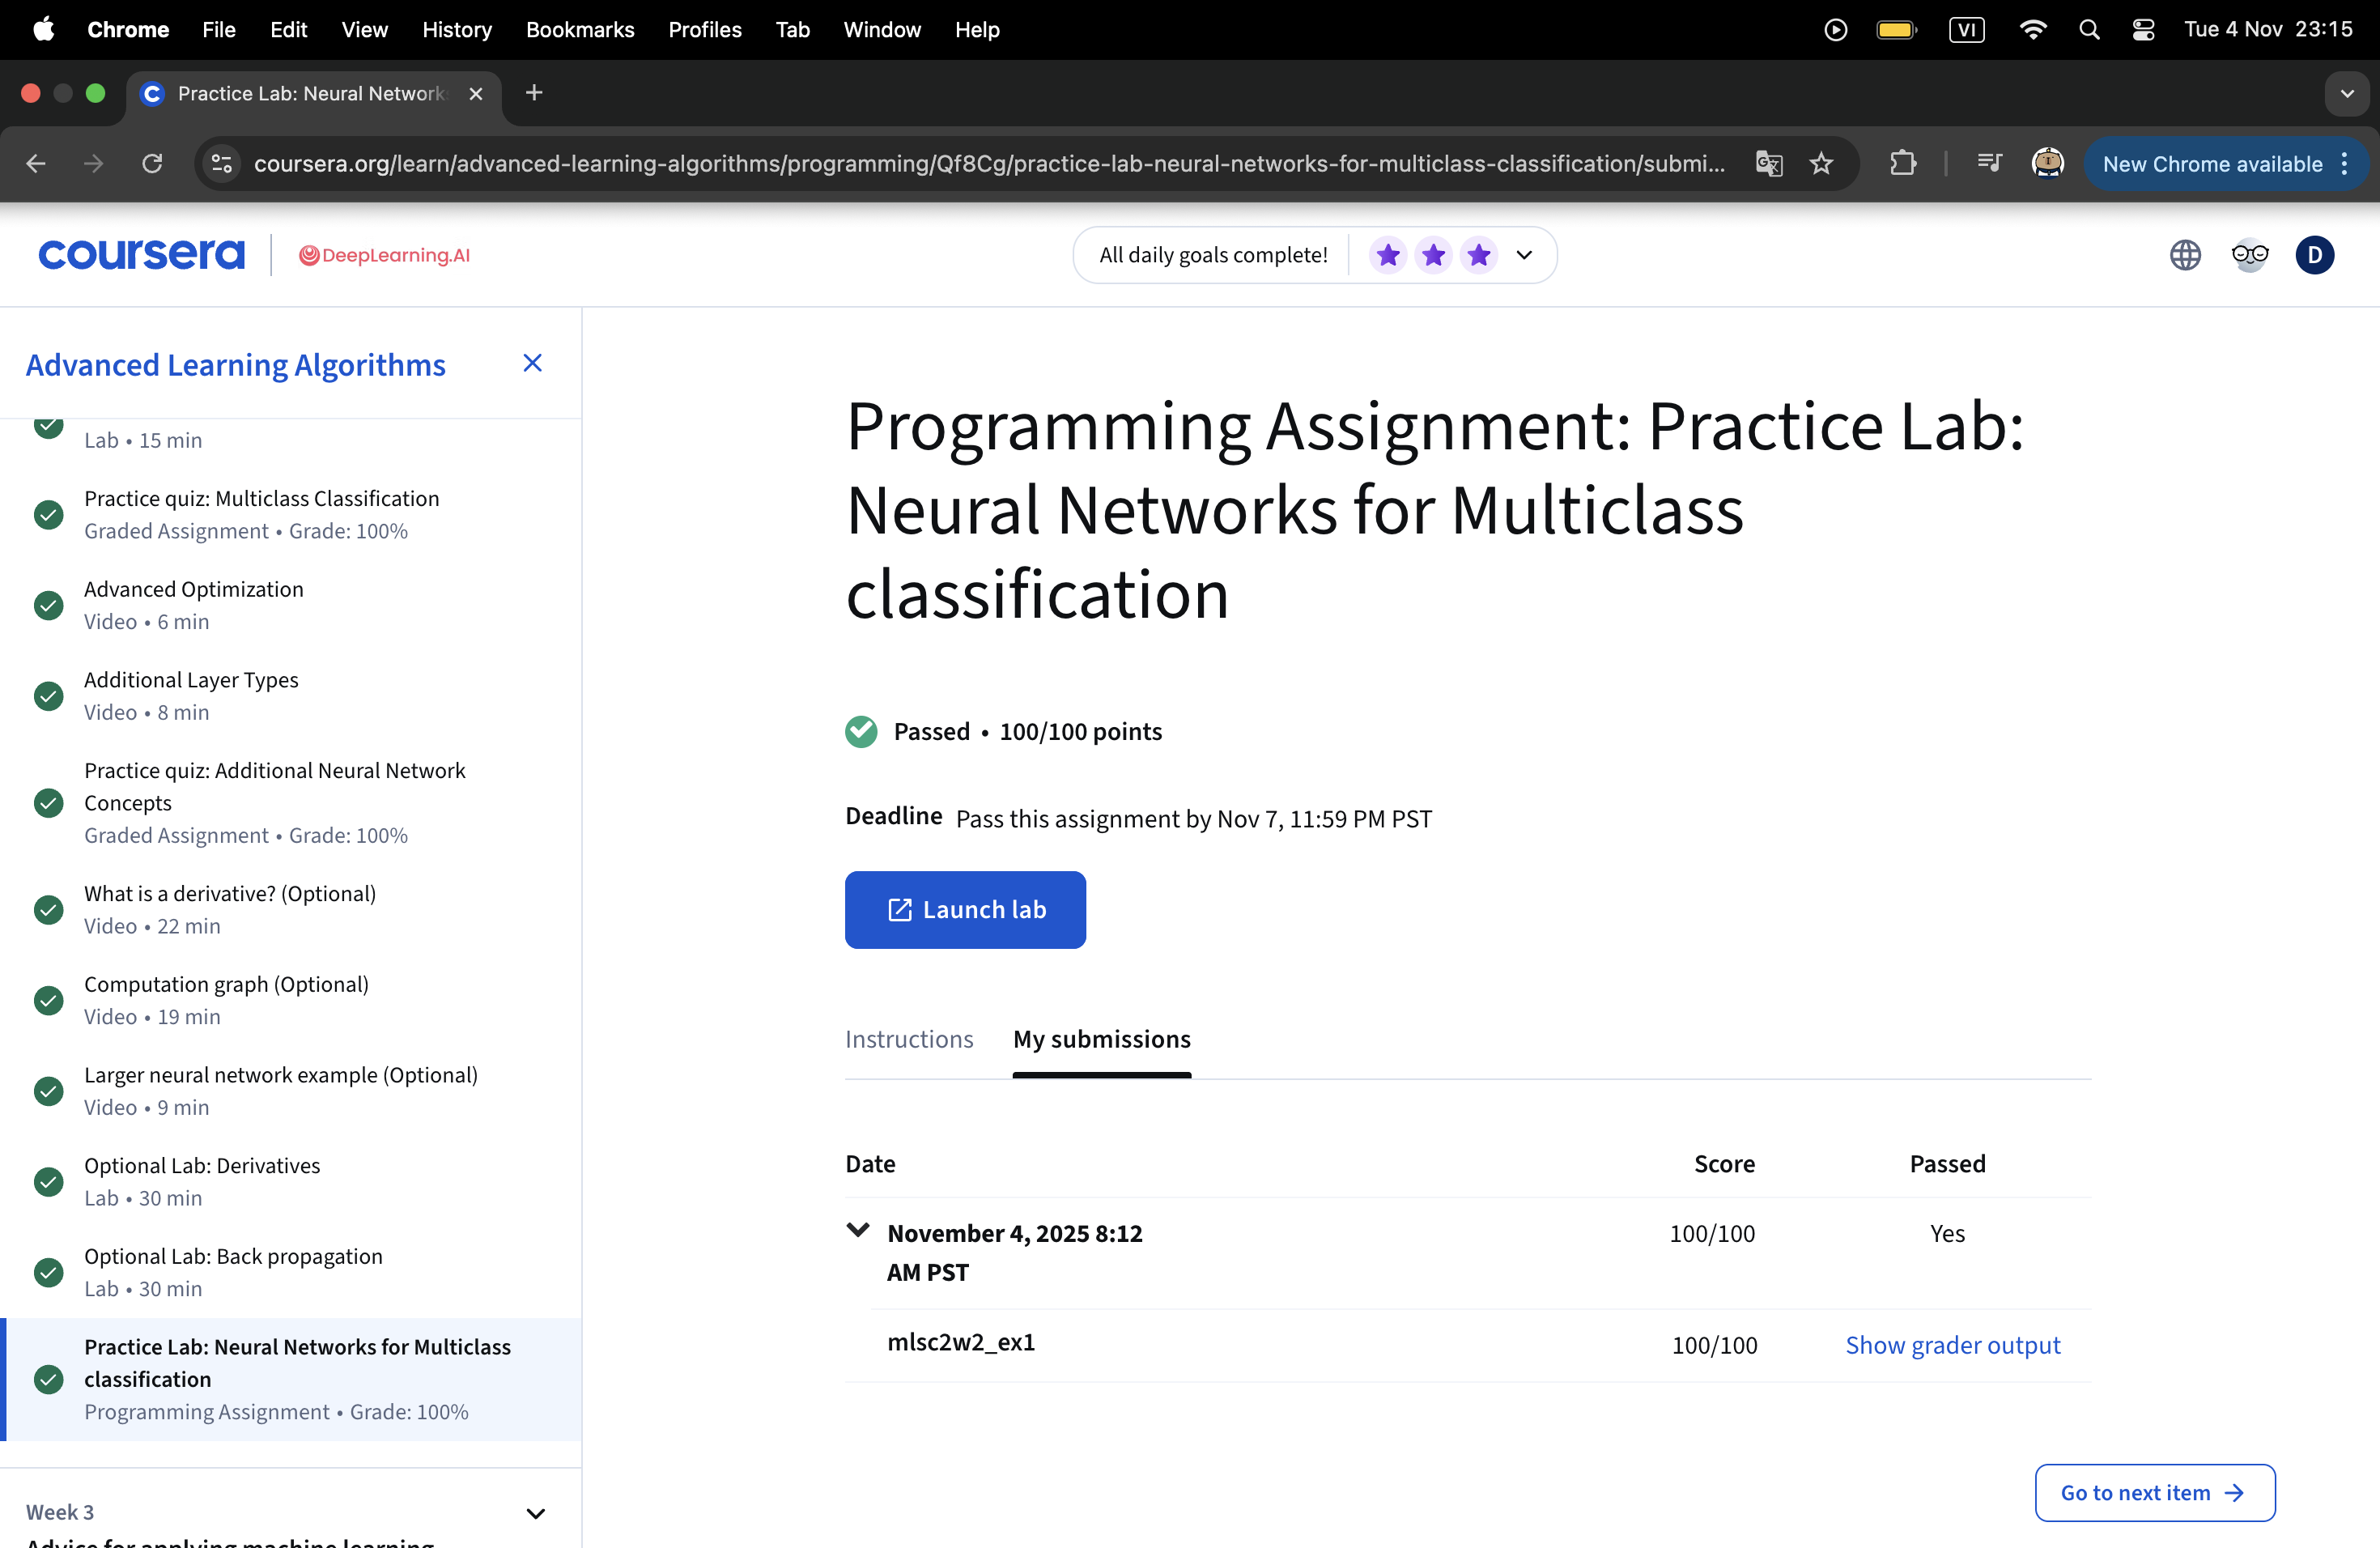
\includegraphics[scale=0.27]{Image/c2_w2_q5.png}
    \caption{Completed Programming Assignment (Neural Networks for Multiclass classification)}
\end{figure}

%----------------------------------------
\subsection{Week 3: Advice for Applying Machine Learning}
%----------------------------------------

\subsubsection{Key Insights and Learnings}

Often considered the most valuable part of the specialization, this module provided a strategic framework for diagnosing and improving model performance.

\begin{itemize}
    \item \textbf{Model Diagnostics (Bias vs. Variance):}
    \begin{itemize}
        \item Utilized \textbf{Learning Curves} to visualize training and cross-validation errors.
        \item \textbf{High Bias (Underfitting):} Addressed by increasing model complexity (adding layers/neurons) or reducing regularization.
        \item \textbf{High Variance (Overfitting):} Addressed by collecting more data or adding regularization/dropout.
    \end{itemize}
    
    \item \textbf{Error Metrics for Skewed Datasets:} Learned that accuracy is misleading for imbalanced classes (e.g., rare disease detection). Adopted \textbf{Precision, Recall}, and the \textbf{F1-Score} as robust evaluation metrics.
    
    \item \textbf{Iterative Loop of ML Development:} Embraced the cycle of \texttt{Idea -> Code -> Experiment}. The systematic split of data into \textbf{Train/Dev (Cross-Validation)/Test} sets is crucial for unbiased tuning.
\end{itemize}

\subsubsection{Learning Evidence}
\begin{figure}[H]
    \centering
    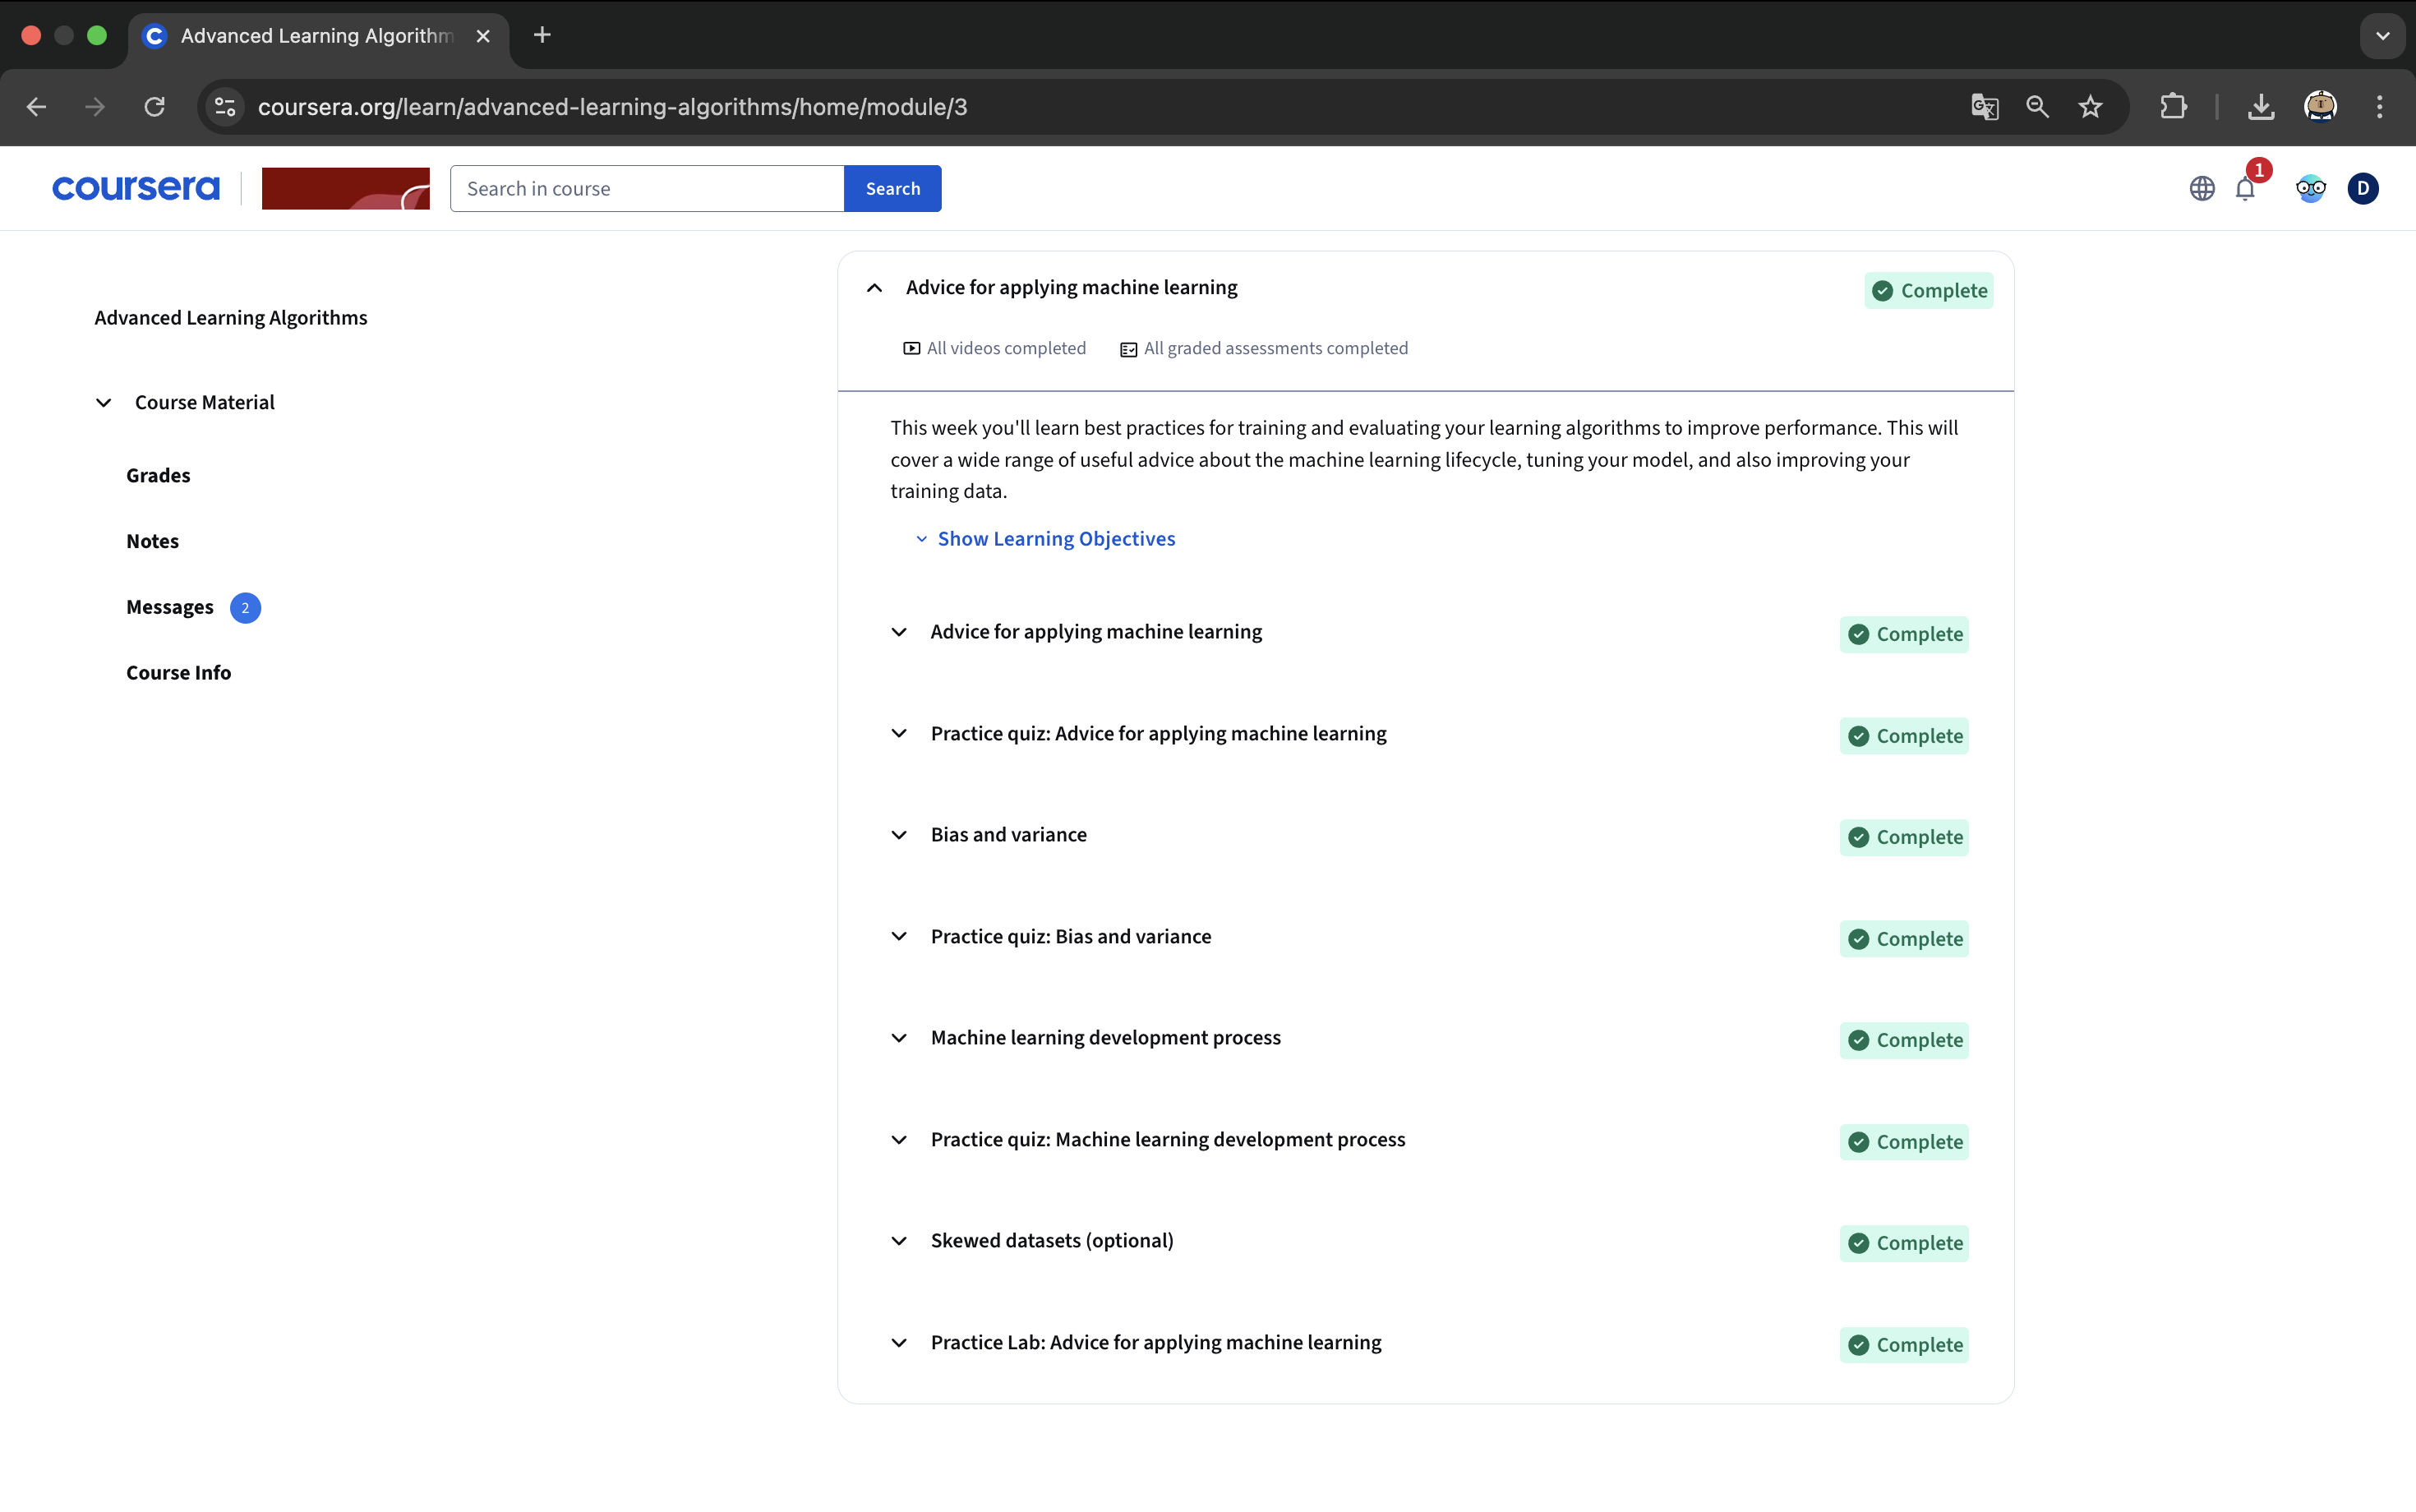
\includegraphics[scale=0.27]{Image/c2_w3.png}
    \caption{Lesson's completed date (07/11/2025)}
\end{figure}

\subsubsection{Graded Assignment Evidence}
\begin{figure}[H]
    \centering
    
\includegraphics[scale=0.25]{Image/c2_w3_q1.png}
    \caption{Completed Graded Assignment 1 (Advice for applying machine learning)}
\end{figure}

\begin{figure}[H]
    \centering
    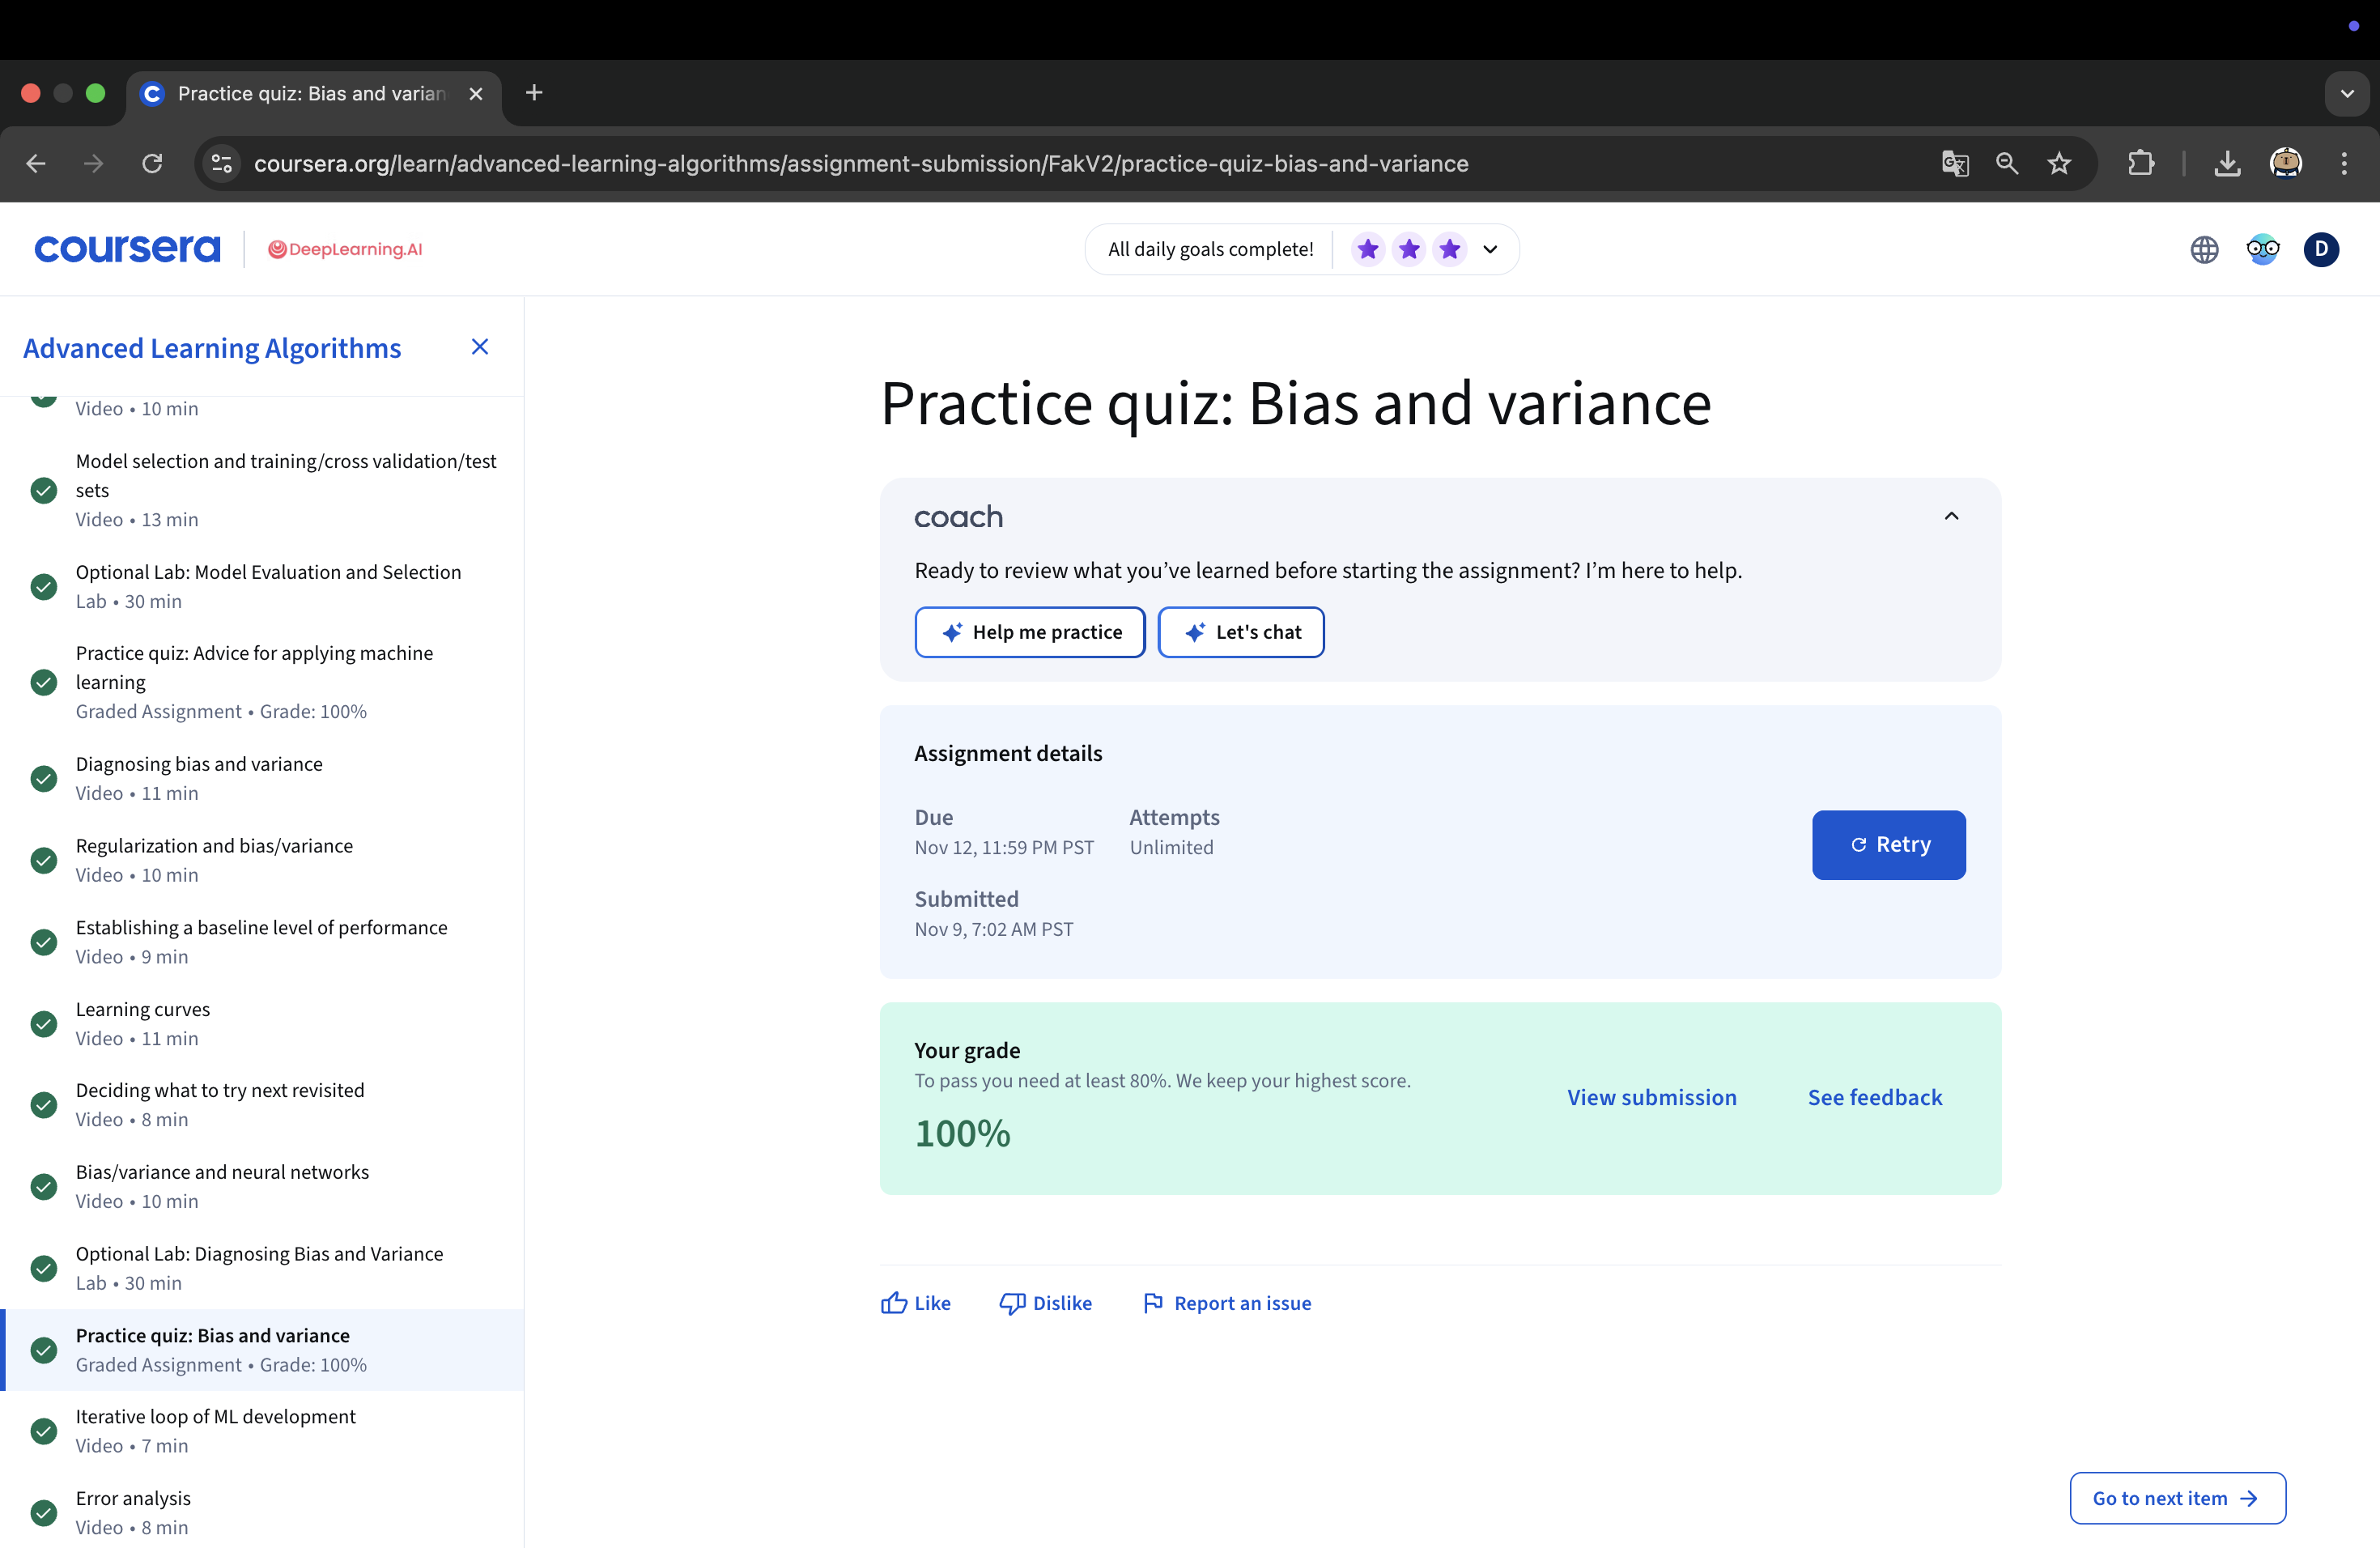
\includegraphics[scale=0.27]{Image/c2_w3_q2.png}
    \caption{Completed Graded Assignment 2 (Bias and variance)}
\end{figure}

\begin{figure}[H]
    \centering
    
\includegraphics[scale=0.27]{Image/c2_w3_q3.png}
    \caption{Completed Graded Assignment 3 (Machine learning development process)}
\end{figure}

\begin{figure}[H]
    \centering
    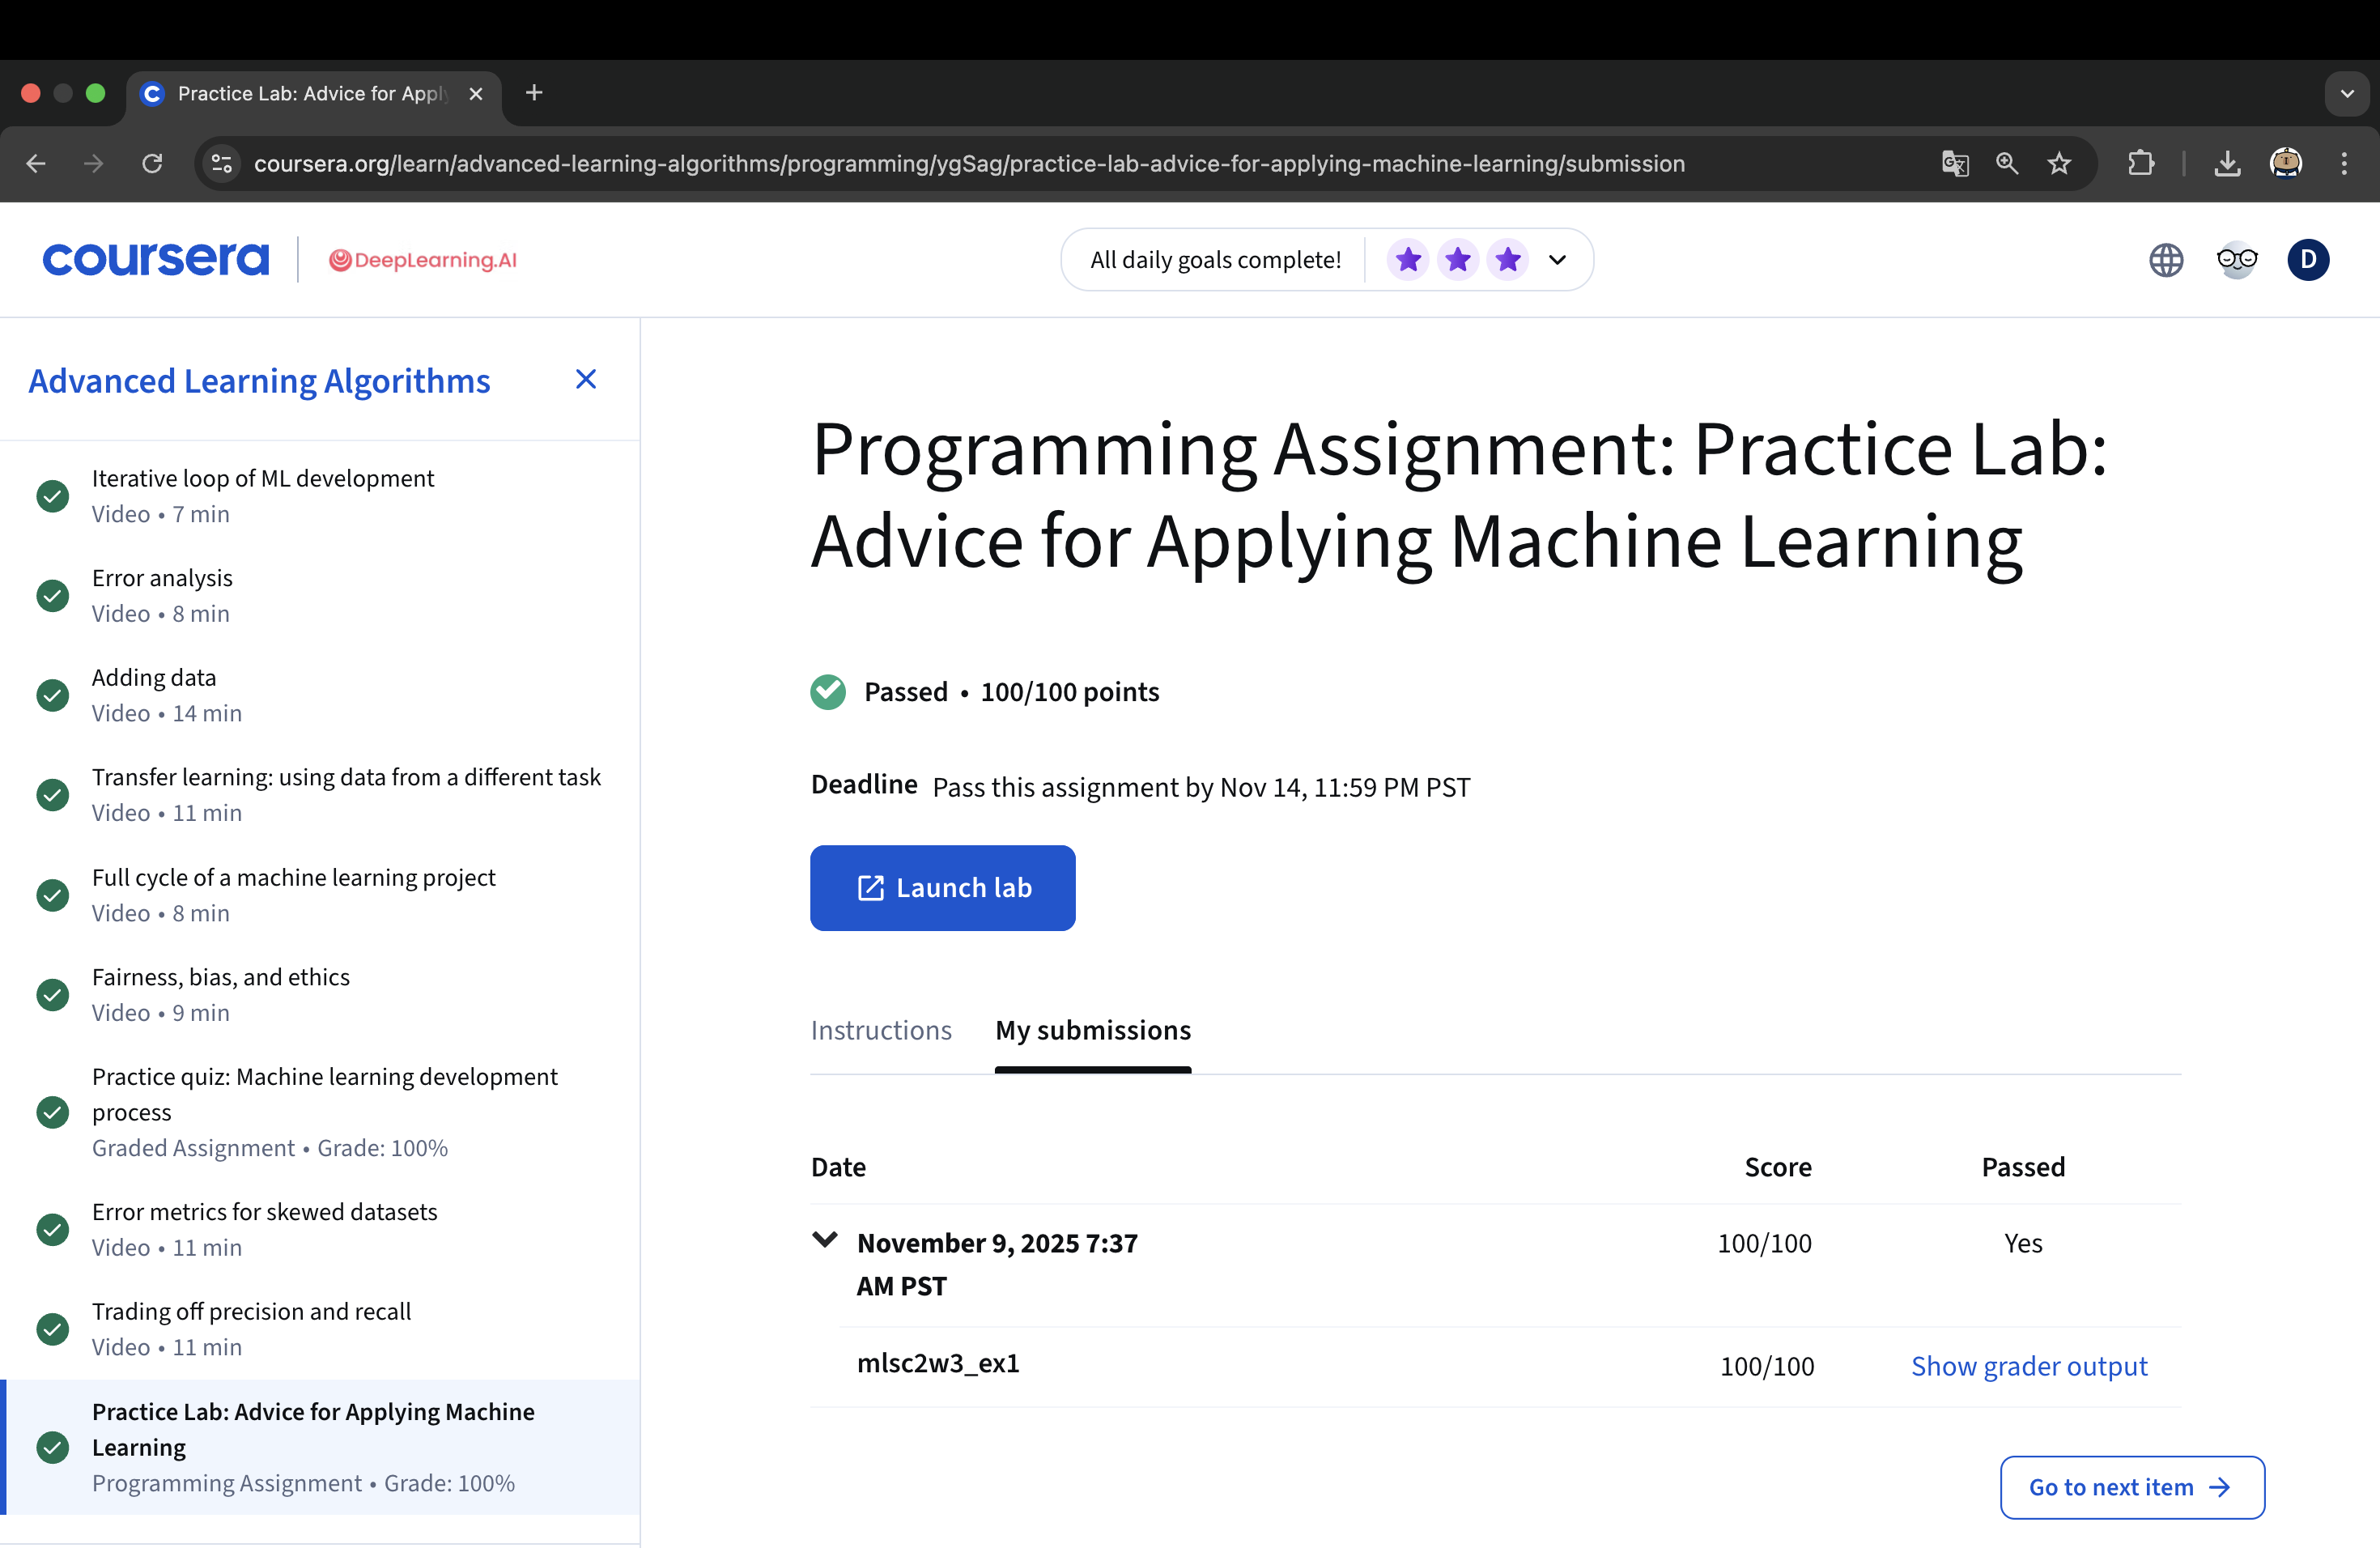
\includegraphics[scale=0.27]{Image/c2_w3_q4.png}
    \caption{Completed Programming Assignment (Advice for Applying Machine Learning)}
\end{figure}

%----------------------------------------
\subsection{Week 4: Decision Trees and Ensemble Methods}
%----------------------------------------

\subsubsection{Key Insights and Learnings}

This module introduced robust alternatives to Neural Networks, particularly effective for structured (tabular) data.

\begin{itemize}
    \item \textbf{Decision Trees Mechanics:}
    \begin{itemize}
        \item The learning process involves recursively splitting data to maximize \textbf{Information Gain} (reducing Entropy).
        \item Highly interpretable models where decision paths can be visualized and explained to non-technical stakeholders.
    \end{itemize}
    
    \item \textbf{Ensemble Methods (The Wisdom of Crowds):}
    \begin{itemize}
        \item \textbf{Random Forests (Bagging):} Builds multiple trees on random subsets of data (sampling with replacement). It averages predictions to reduce \textbf{variance} and prevent overfitting.
        \item \textbf{XGBoost (Boosting):} A state-of-the-art algorithm that trains trees sequentially. Each new tree focuses on correcting the residual errors of the previous ones. It is currently the industry standard for tabular data competitions (e.g., Kaggle).
    \end{itemize}
\end{itemize}

\subsubsection{Learning Evidence}
\begin{figure}[H]
    \centering
    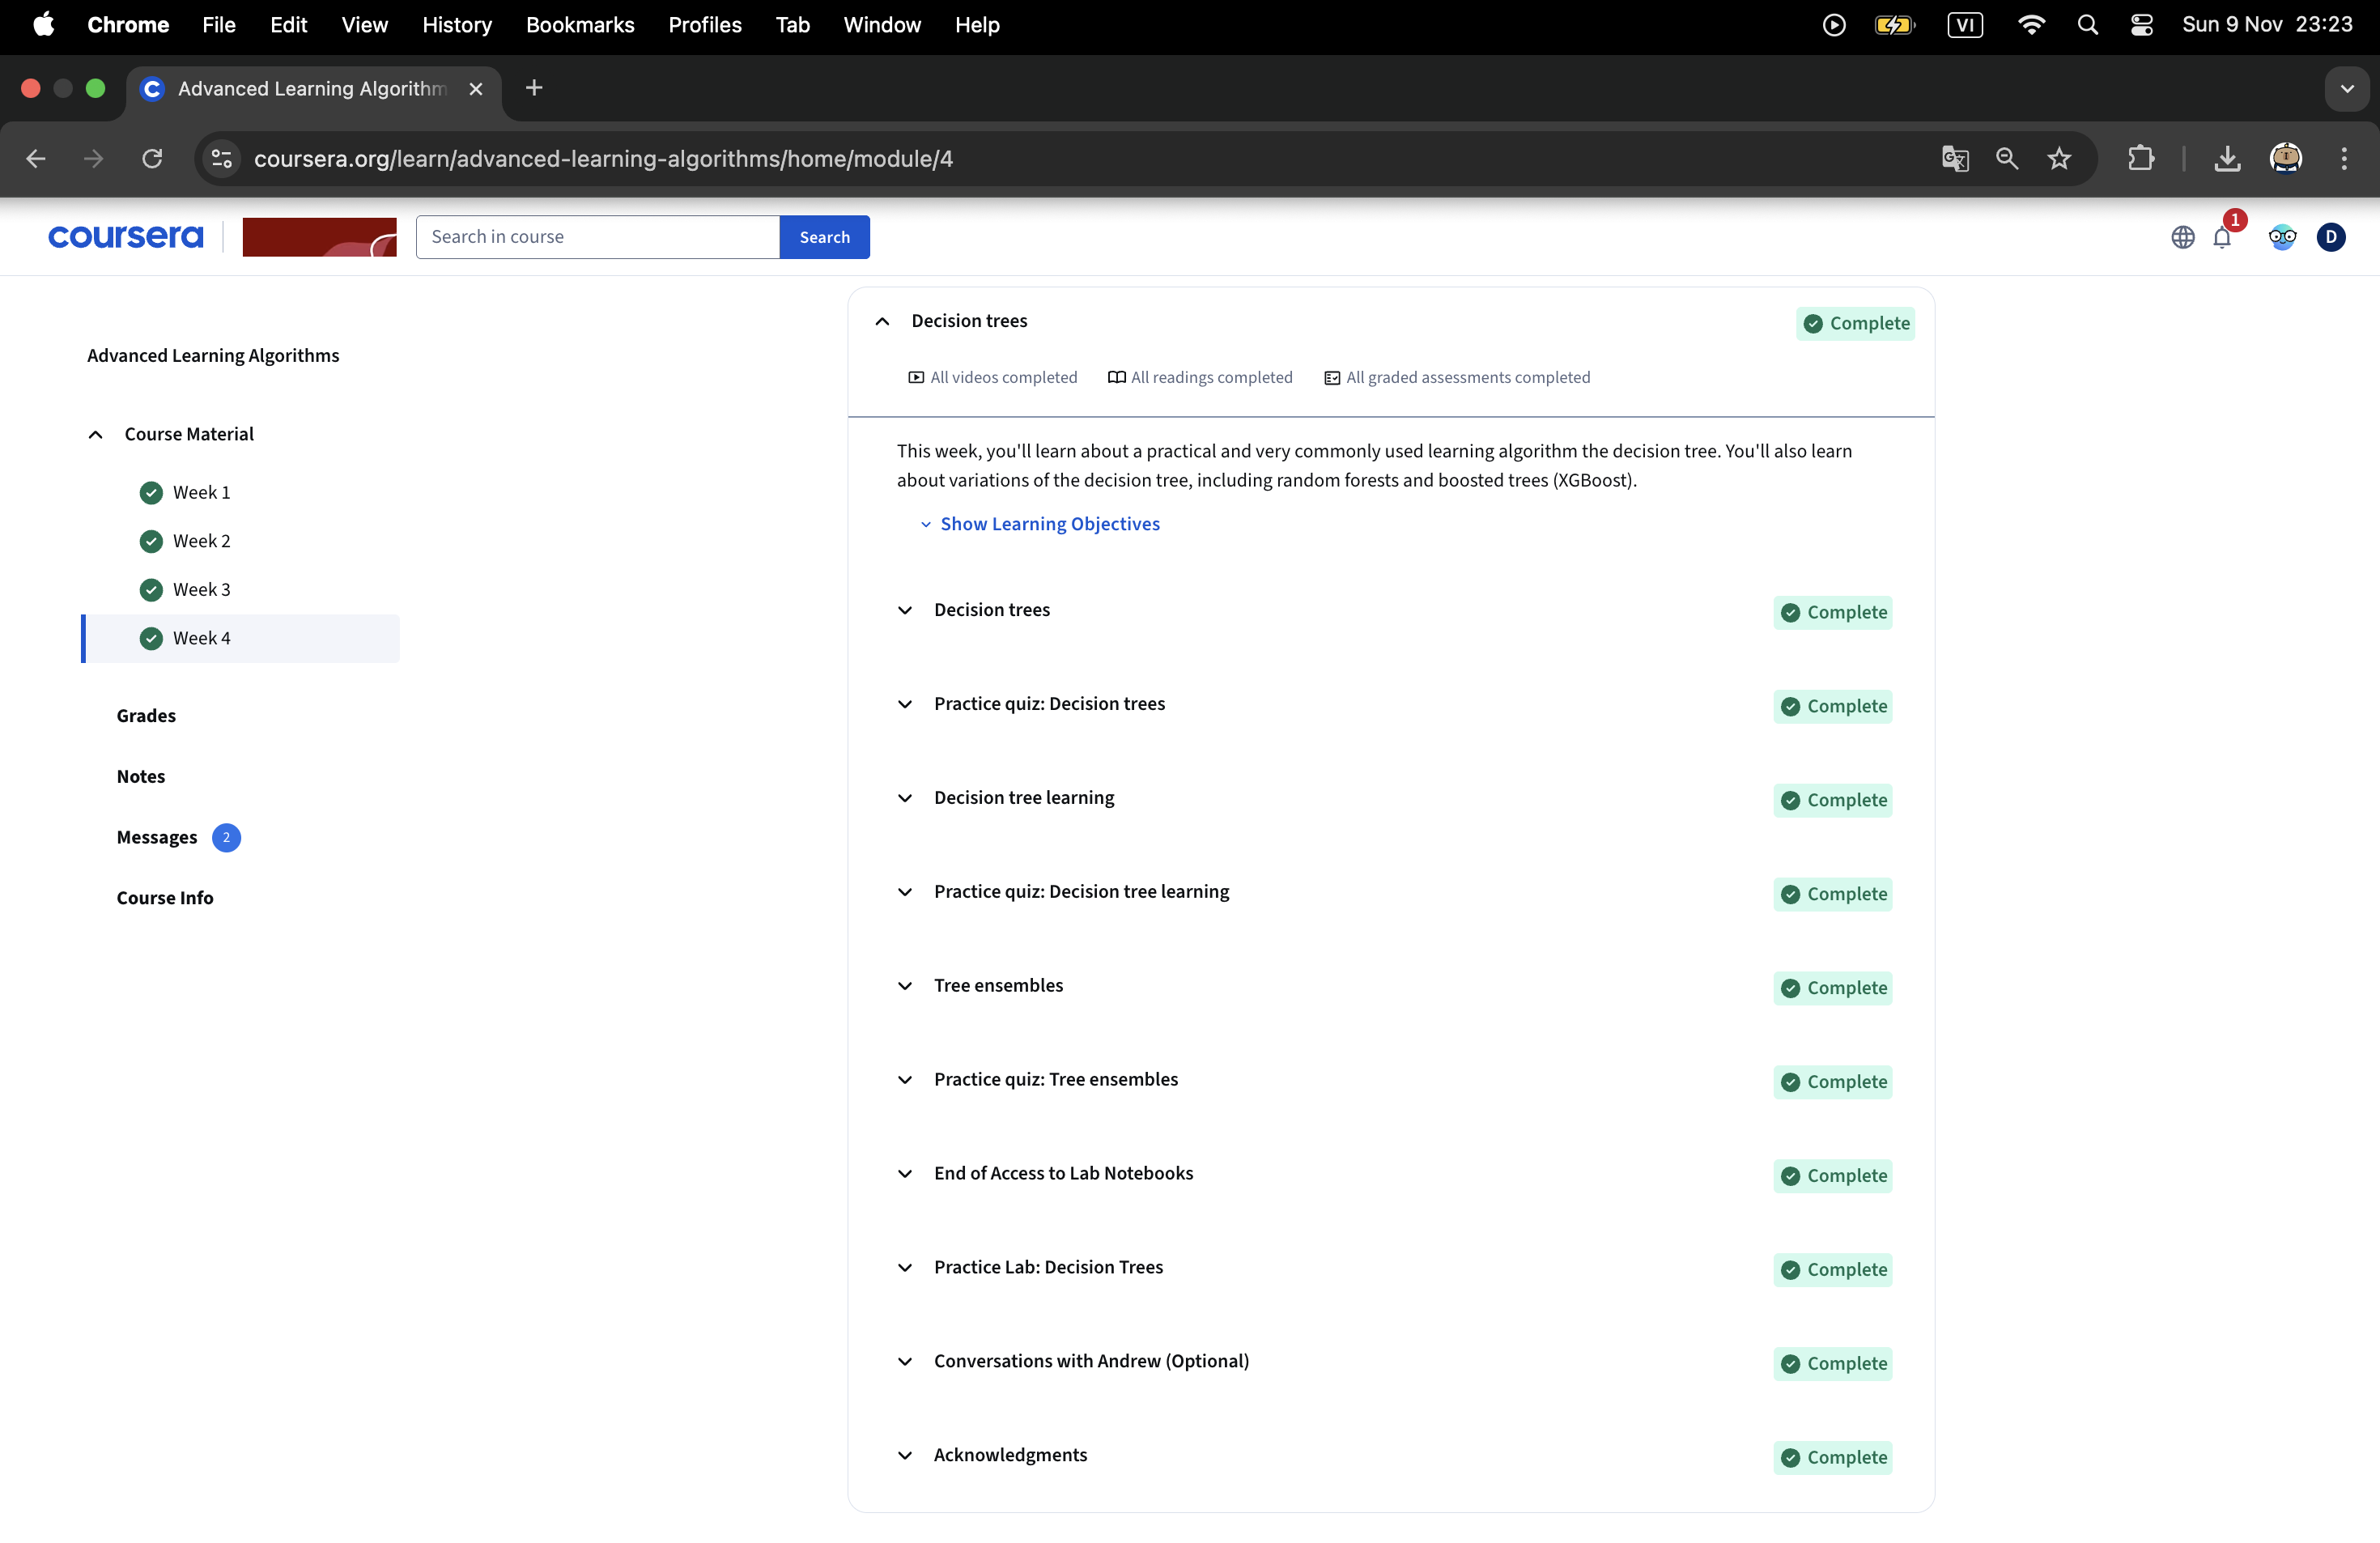
\includegraphics[scale=0.25]{Image/c2_w4.png}
    \caption{Lesson's completed date (09/11/2025)}
\end{figure}

\subsubsection{Graded Assignment Evidence}
\begin{figure}[H]
    \centering
    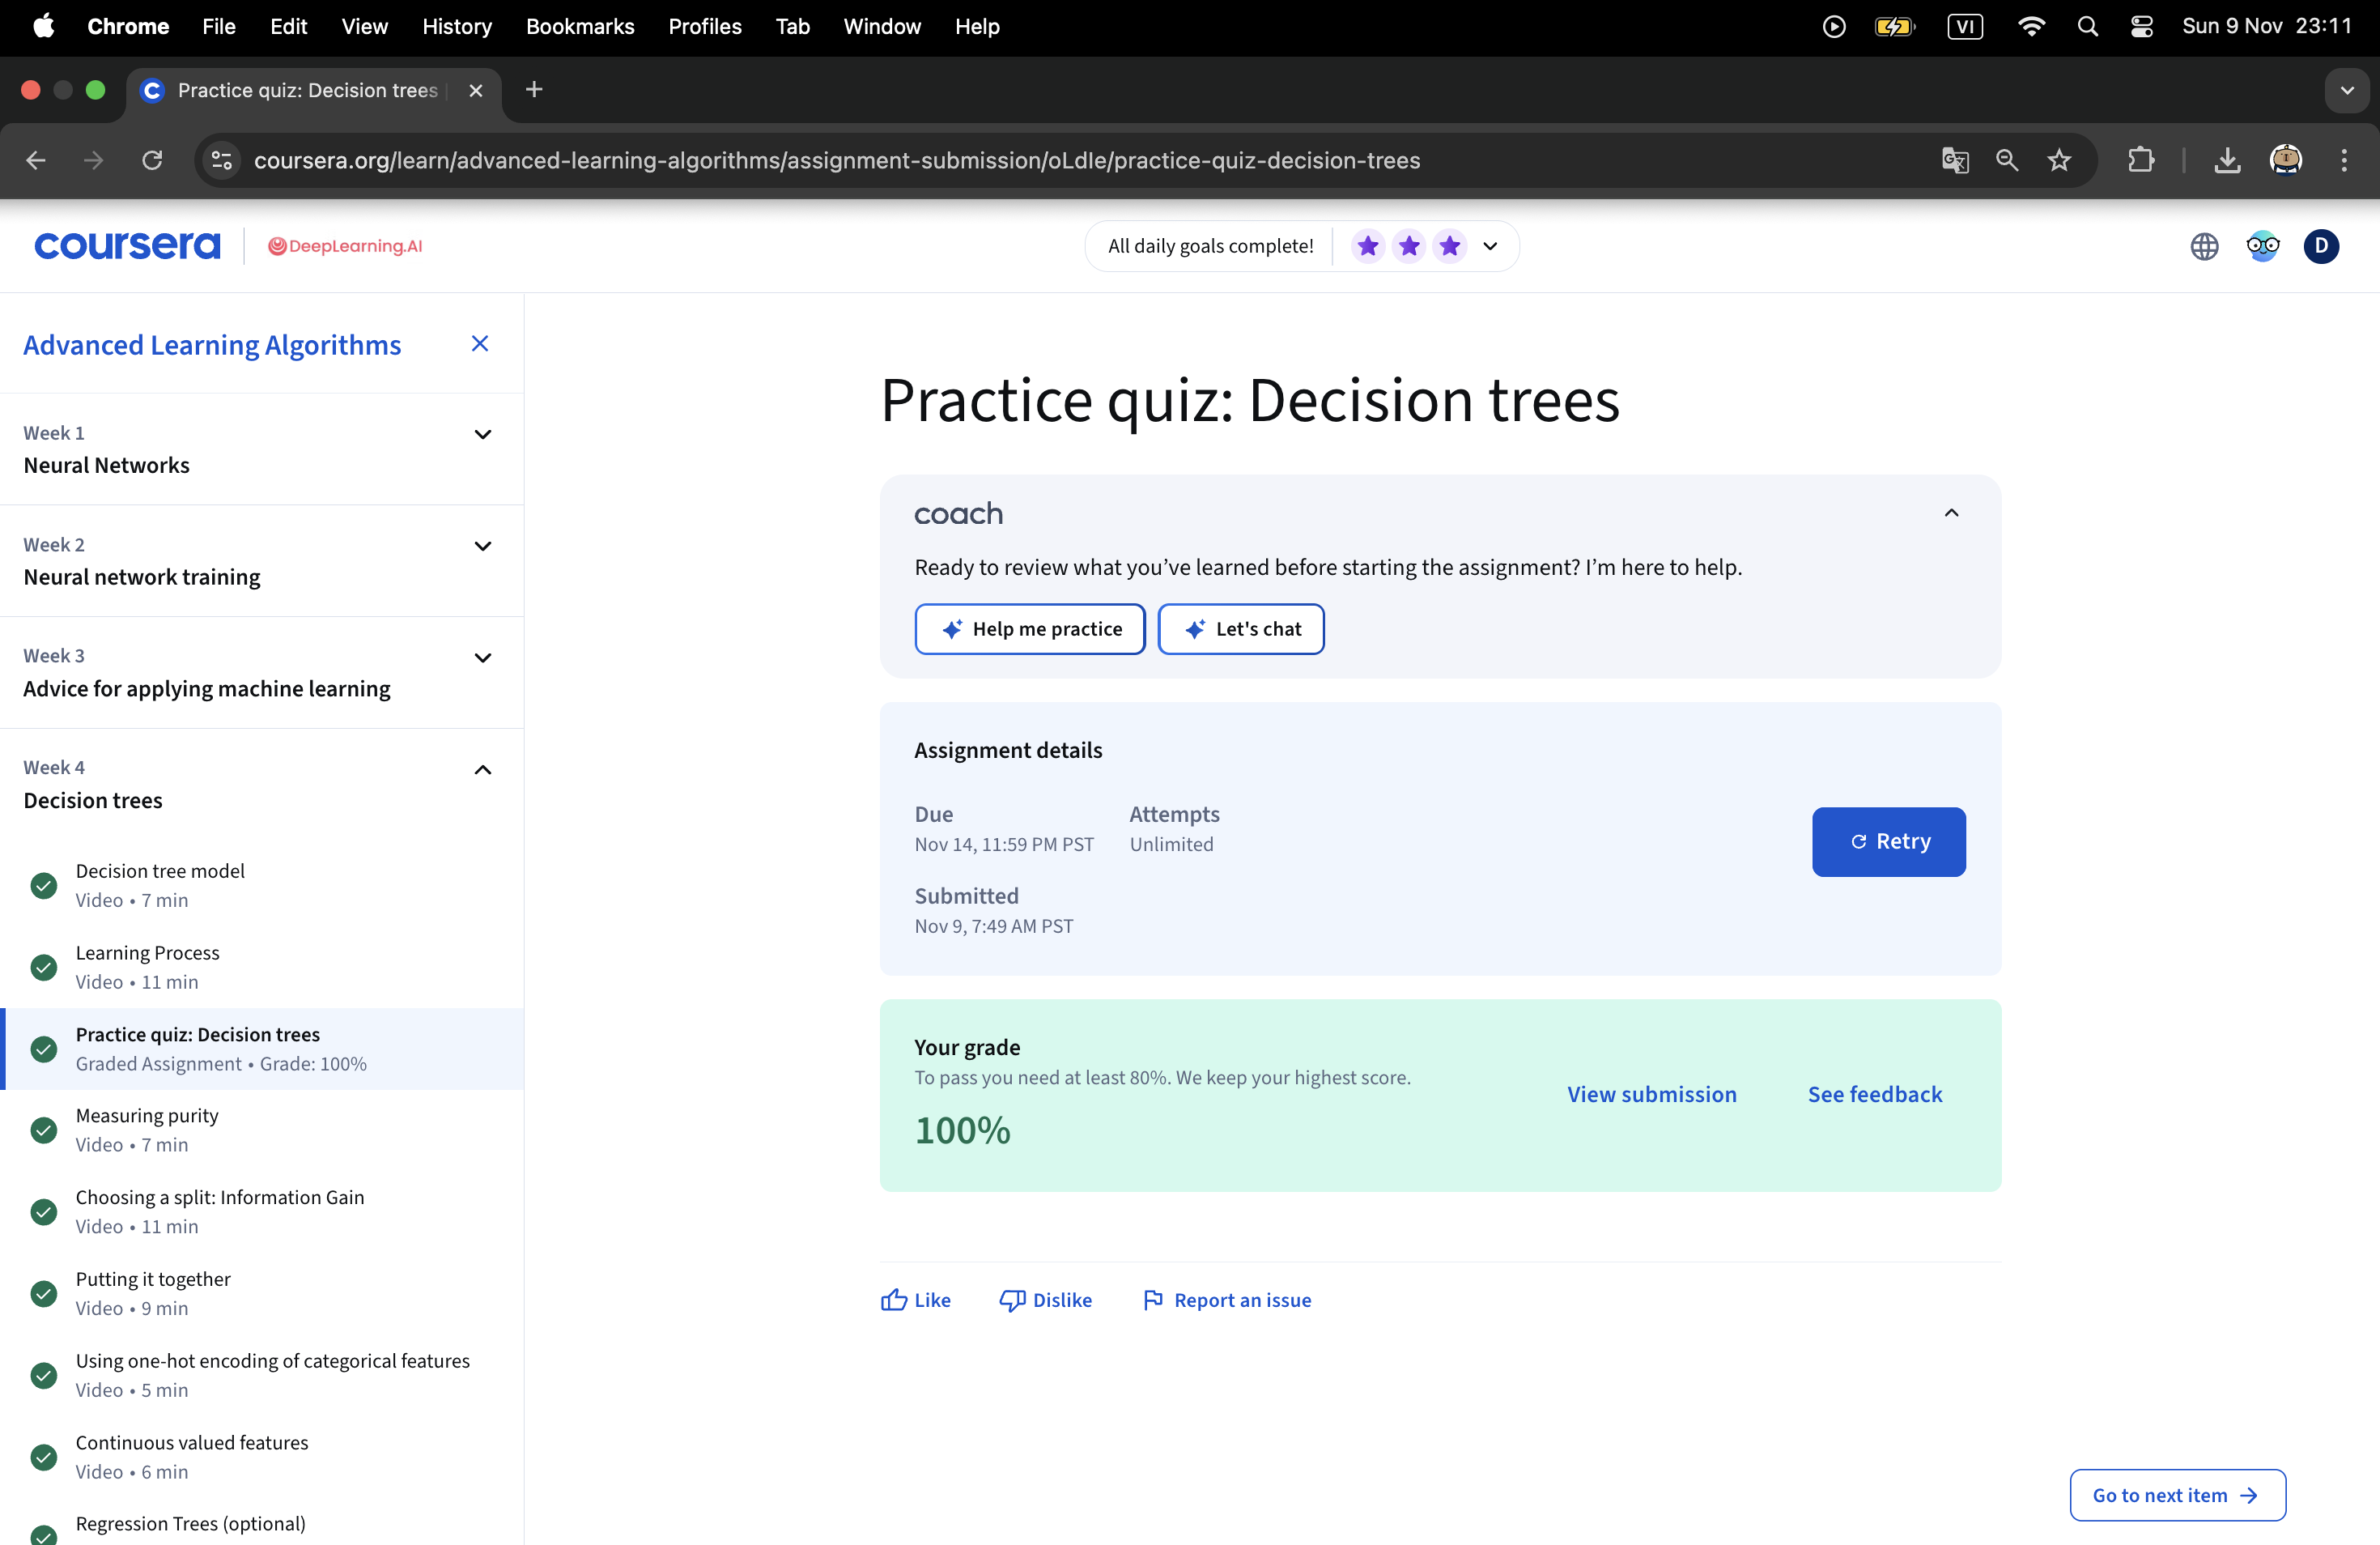
\includegraphics[scale=0.25]{Image/c2_w4_q1.png}
    \caption{Completed Graded Assignment 1 (Decision trees)}
\end{figure}

\begin{figure}[H]
    \centering
    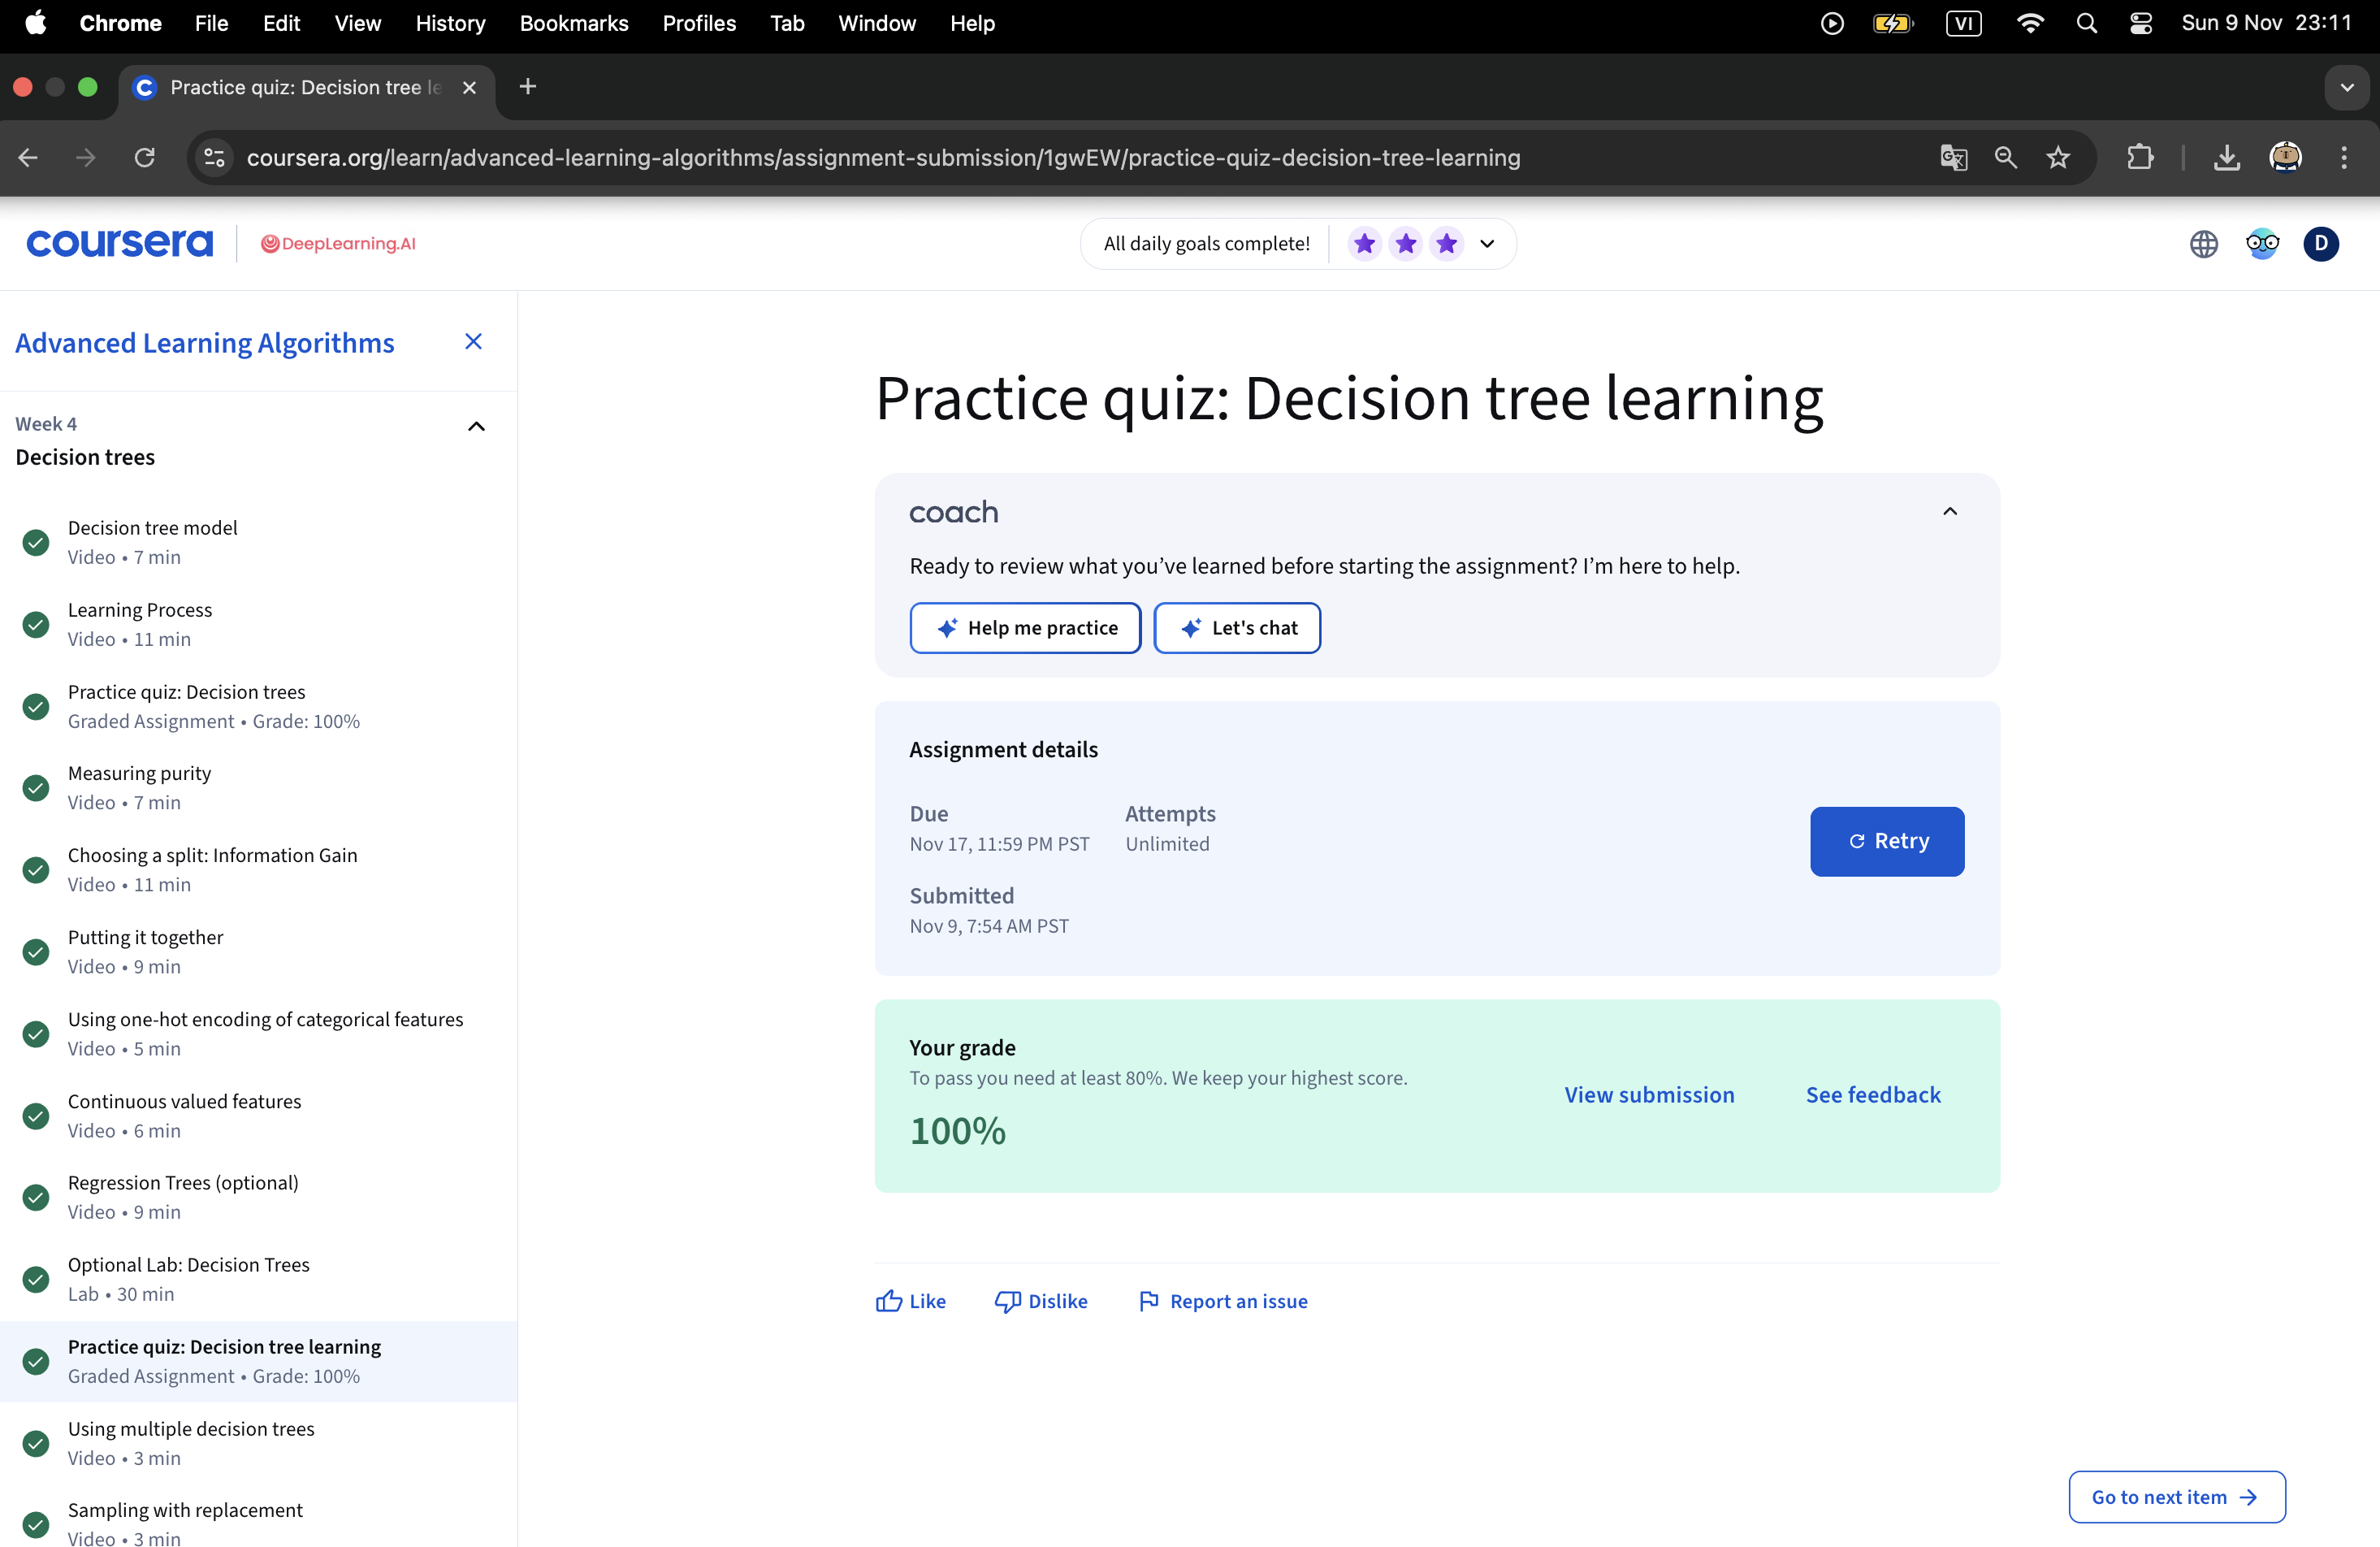
\includegraphics[scale=0.25]{Image/c2_w4_q2.png}
    \caption{Completed Graded Assignment 2 (Decision tree learning)}
\end{figure}

\begin{figure}[H]
    \centering
    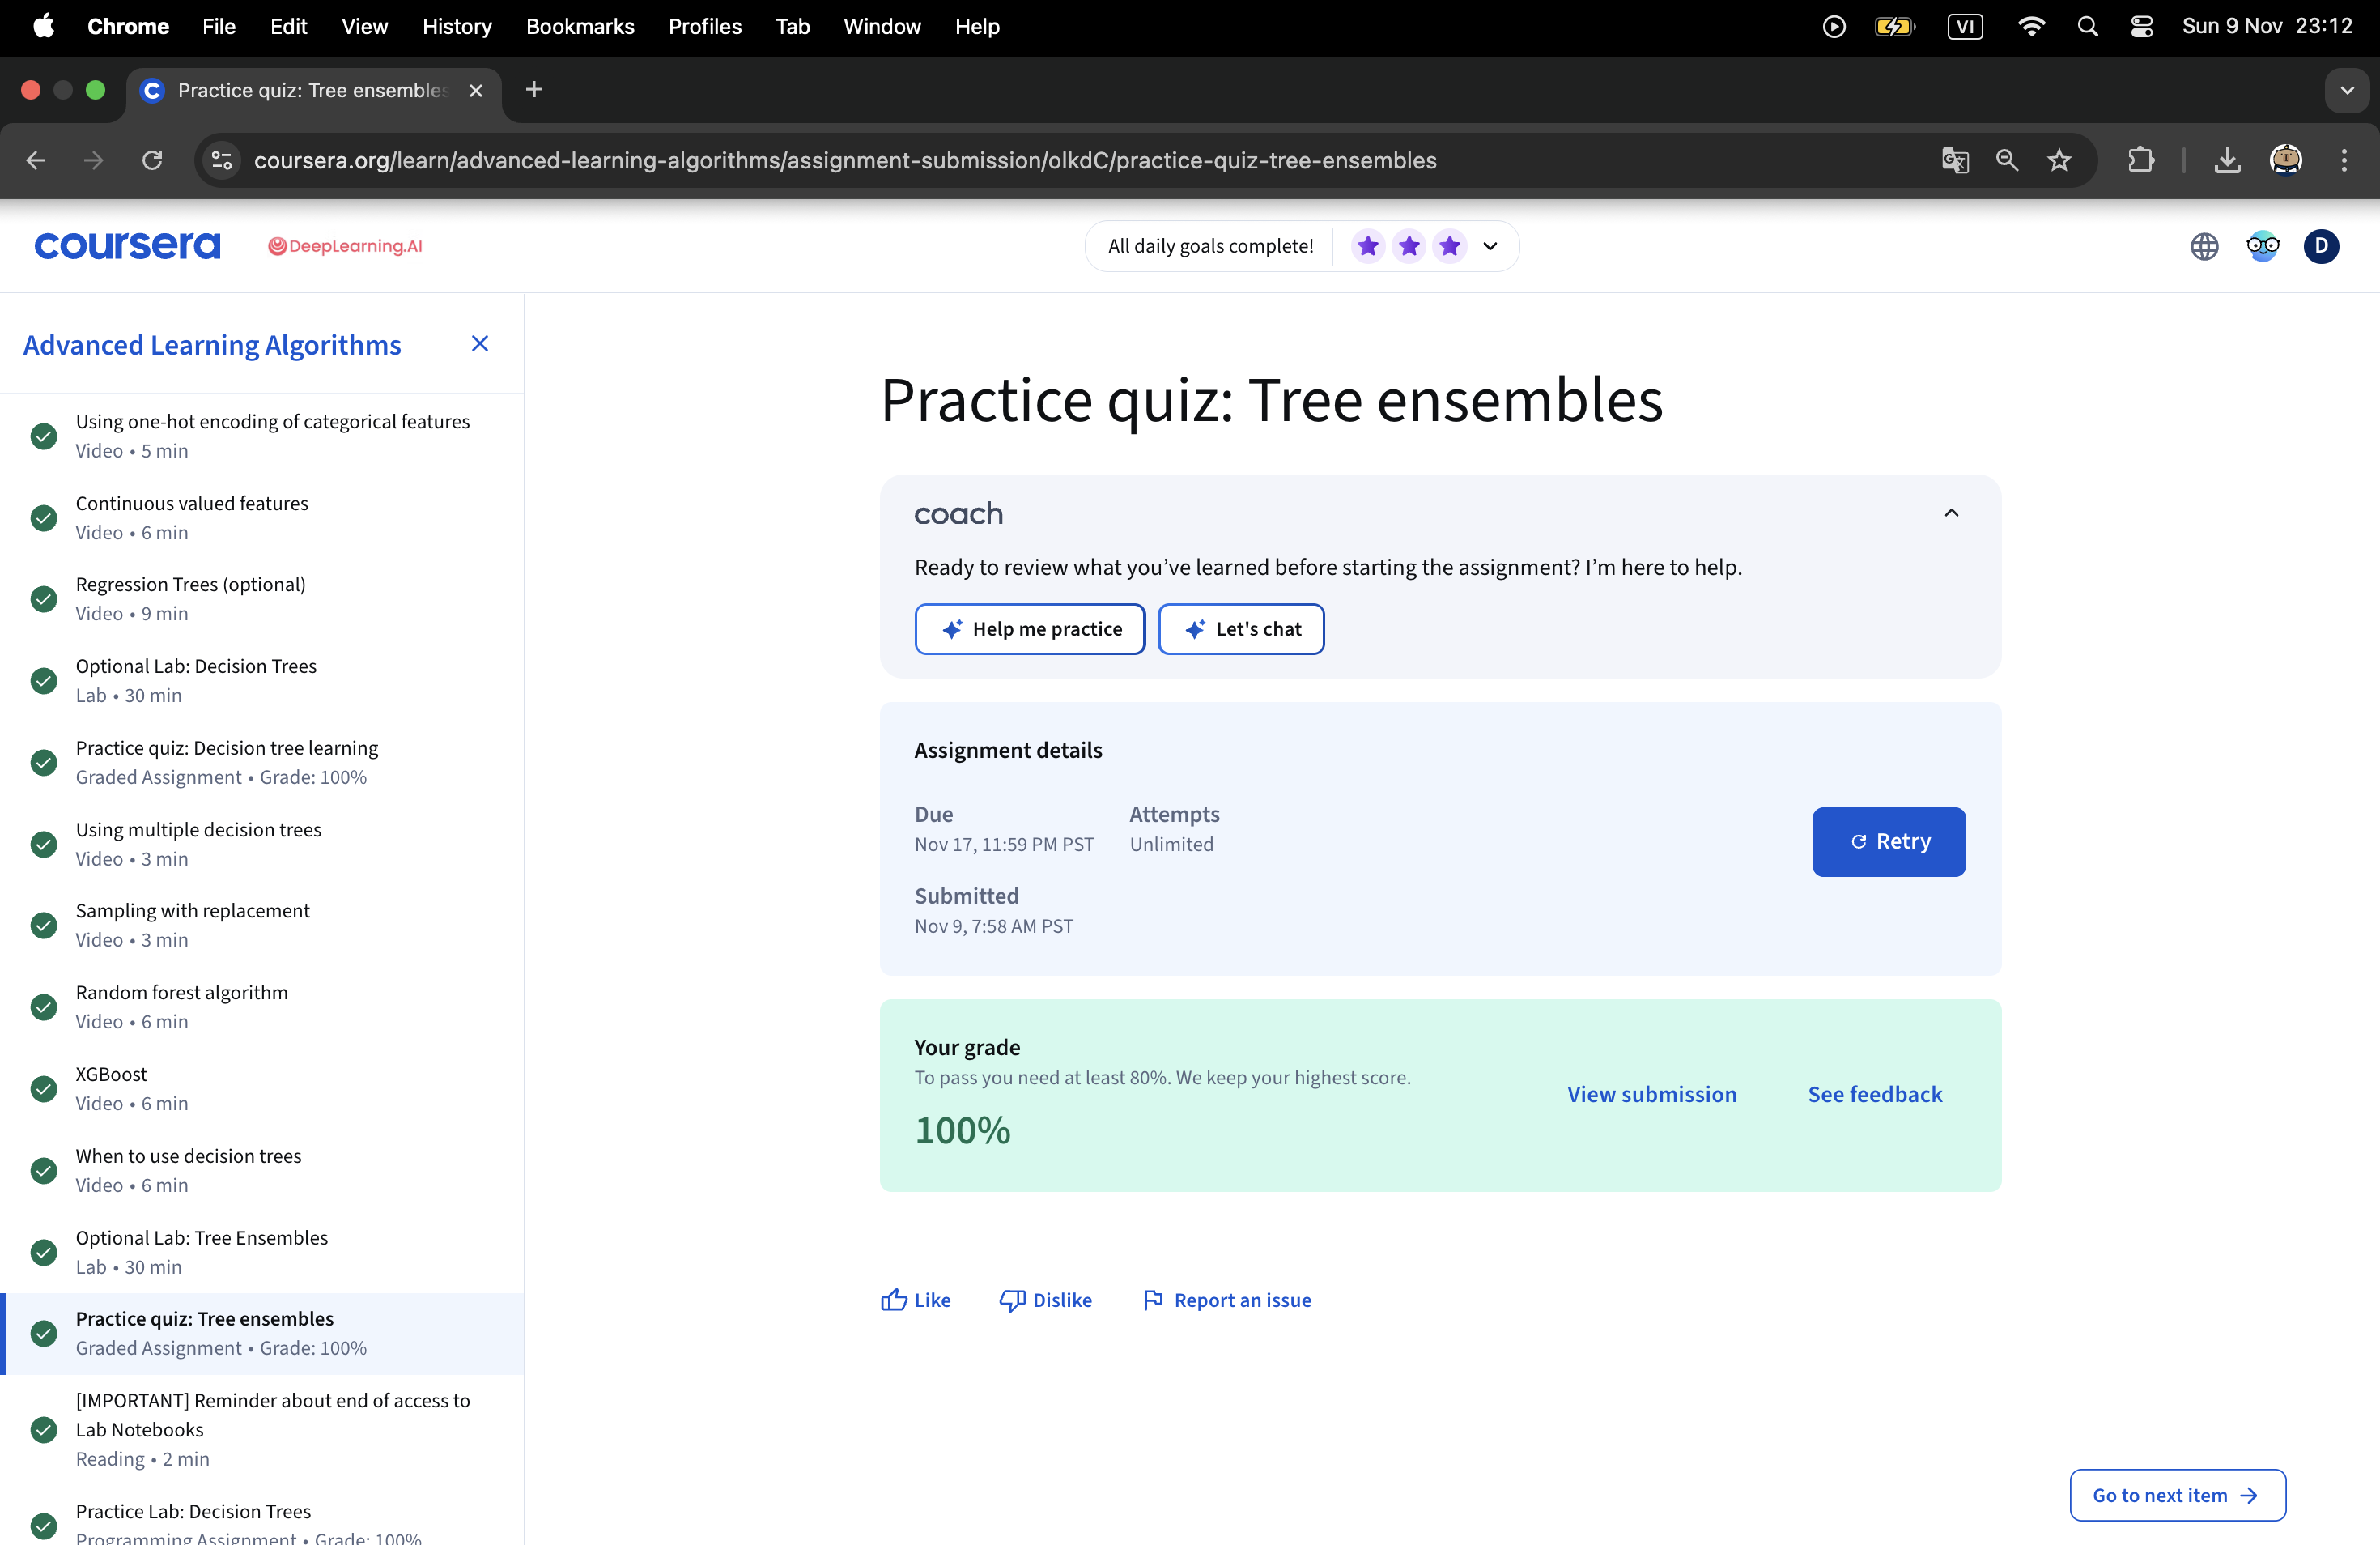
\includegraphics[scale=0.25]{Image/c2_w4_q3.png}
    \caption{Completed Graded Assignment 3 (Tree ensembles)}
\end{figure}


\begin{figure}[H]
    \centering
    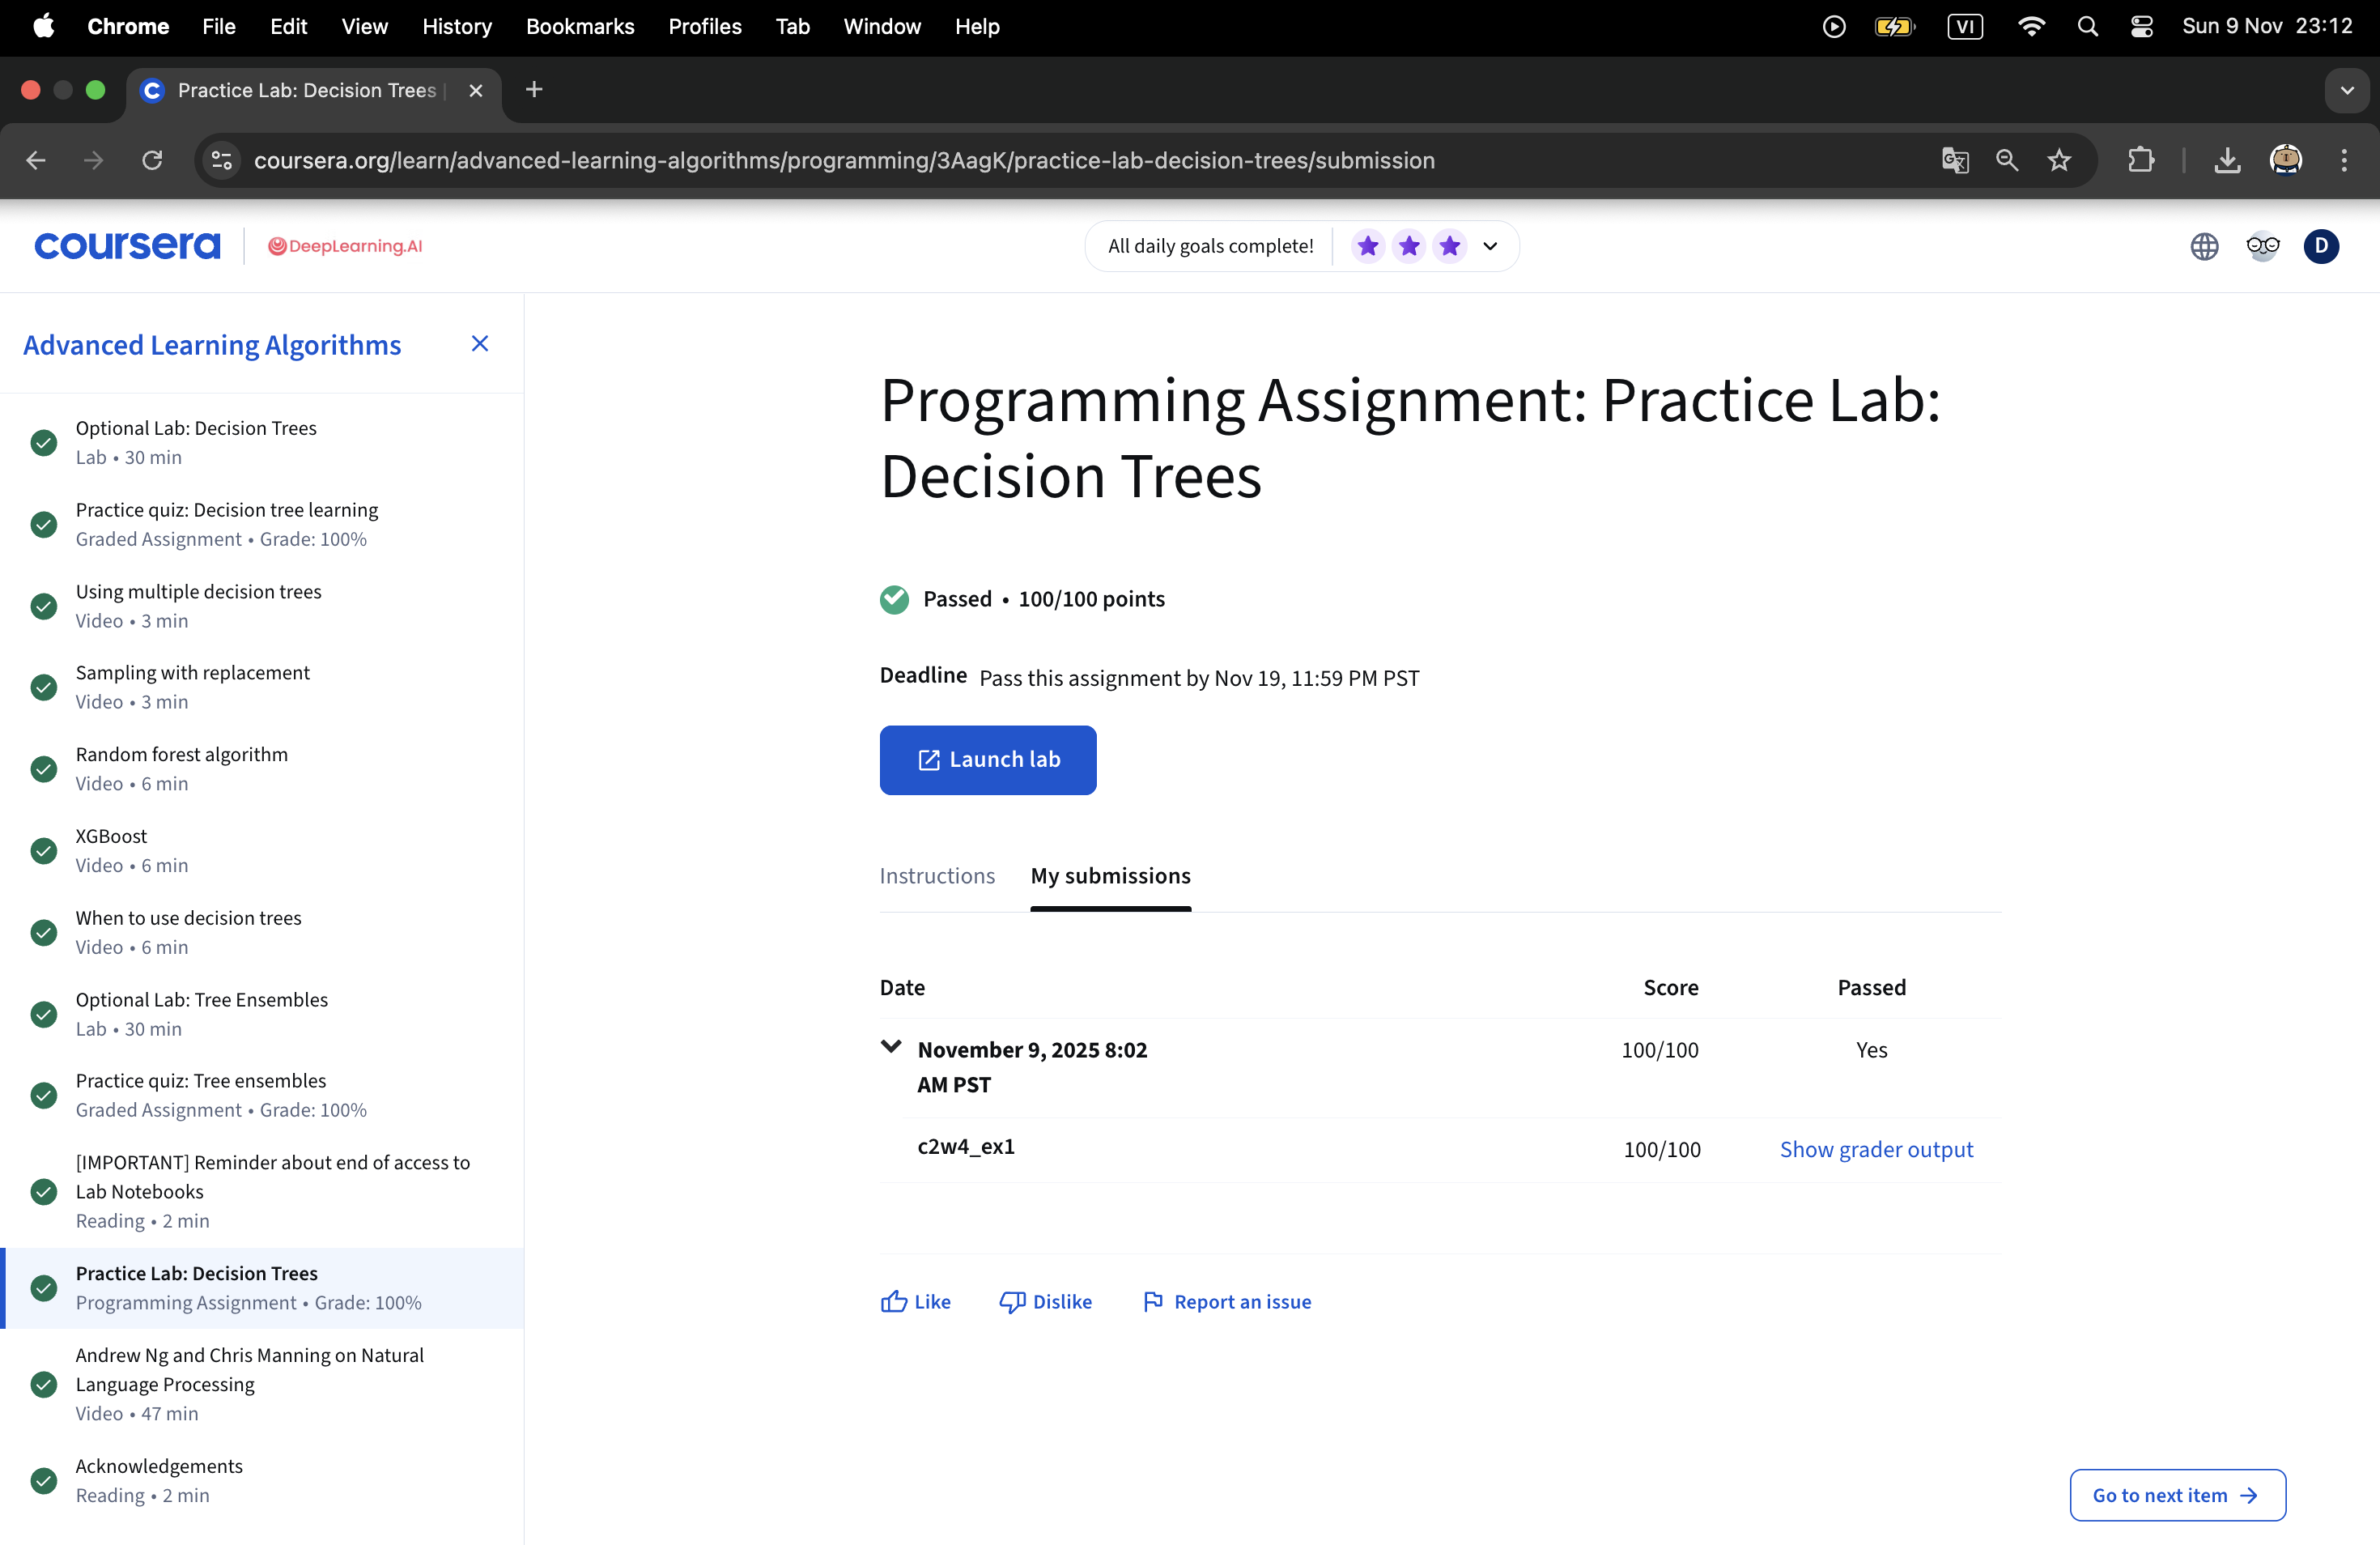
\includegraphics[scale=0.25]{Image/c2_w4_q4.png}
    \caption{Completed Programming Assignment (Decision Trees)}
\end{figure}

\subsection{Certificate for Completion}
\begin{figure}[H]
    \centering
    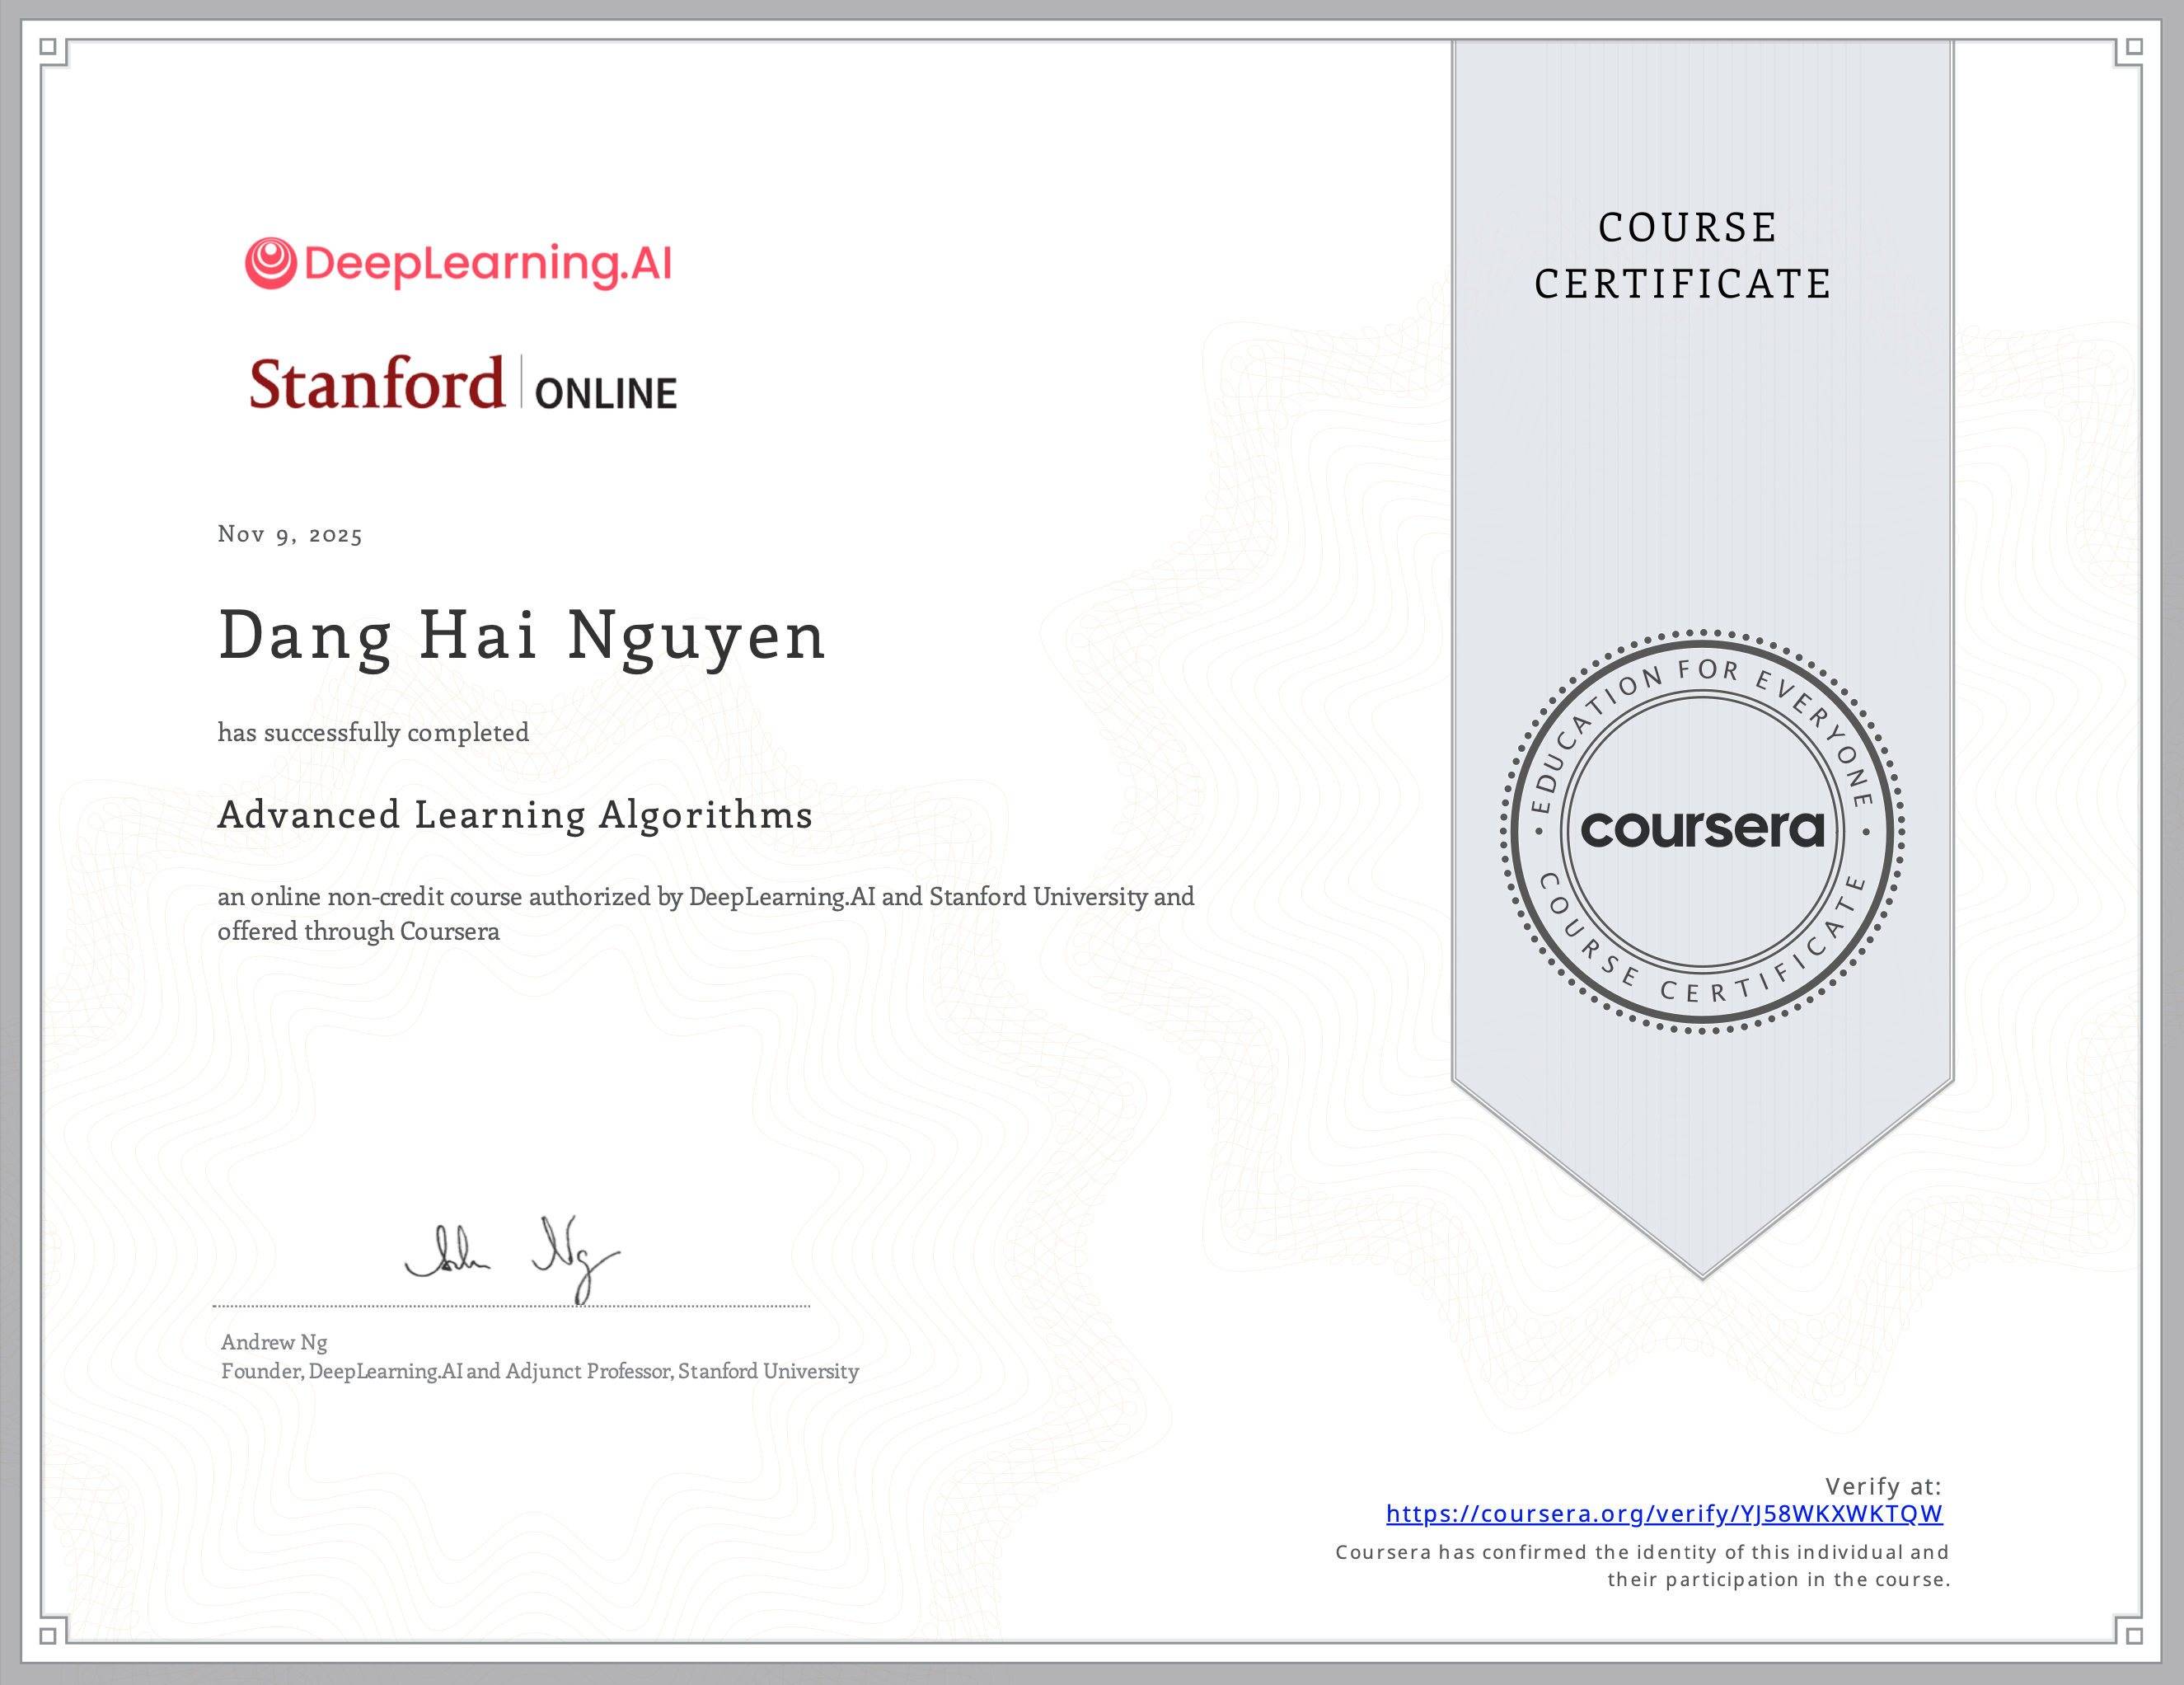
\includegraphics[scale=0.25]{Image/c2_certi.png}
    \caption{Certificate of completion for the course \textit{Advanced Learning Algorithms}.}
\end{figure}

